\newcommand\myeq{\mkern1.5mu{=}\mkern1.5mu}


In this section we will discuss the optimization results of both wind farms, the apparent benefit of coupled turbine layout and design optimization, as well as the benefit of heterogeneous turbine design in a wind farm.
We will first present the results from the 32-turbine circular wind farm optimizations, followed by the 60-turbine Princess Amalia wind farm optimizations. For each wind farm, we present the optimal COE results for each wind shear exponent and spacing multiplier combination (Figs. \ref{circular_results} and \ref{amalia_results}). Each combination has four points, representing a layout optimization performed with the baseline turbine design, a turbine design optimized in isolation followed by layout optimization, coupled layout and homogeneous turbine design optimization, and finally coupled layout and turbine design optimization with two different turbine groups. 
We next show the optimal rotor diameters and hub heights of the turbines optimized in isolation (Figs. \ref{circular_turbines_seq} and \ref{amalia_turbines_seq}), the rotor diameters and hub heights of the coupled design-and-layout optimization, with homogeneous turbine design (Figs. \ref{circular_turbines_1} and \ref{amalia_turbines_1}), the rotor diameters and hub heights of the coupled design-and-layout optimization, with two different turbine groups (Figs. \ref{circular_turbines} and \ref{amalia_turbines}), and the optimal rated powers of the coupled design-and-layout optimization, for the optimizations with both one and two turbine groups (Figs. \ref{circular_power} and \ref{amalia_power}).
% Figures \ref{circular_turbines} and \ref{amalia_turbines} show the turbine heights and rotor diameters in the optimization cases with two different turbine groups. Figures \ref{circular_power} and \ref{amalia_power} show the optimal power rating of each turbine group in the optimization cases with two different height groups. 



\subsection{Circular Wind Farm Optimization}

Figure \ref{circular_results} shows the optimal COE results for the circular wind farm. As shown in the legend, the white points represent the layout-only optimization, the gray indicate the sequential-turbine-design-then-layout optimization, the black points show the coupled-turbine-design-and-layout optimization, and the half blue and pink points represent the couple design and layout optimization with two turbine groups.  As expected, the general trends for all optimizations run show that the higher wind speed from high wind shear results in a lower, superior optimal COE. Additionally, the widely spaced wind turbines indicated by the larger spacing multipliers also result in lower COE due to less wake interaction between turbines. 

\begin{figure}[htbp]
  \centering
  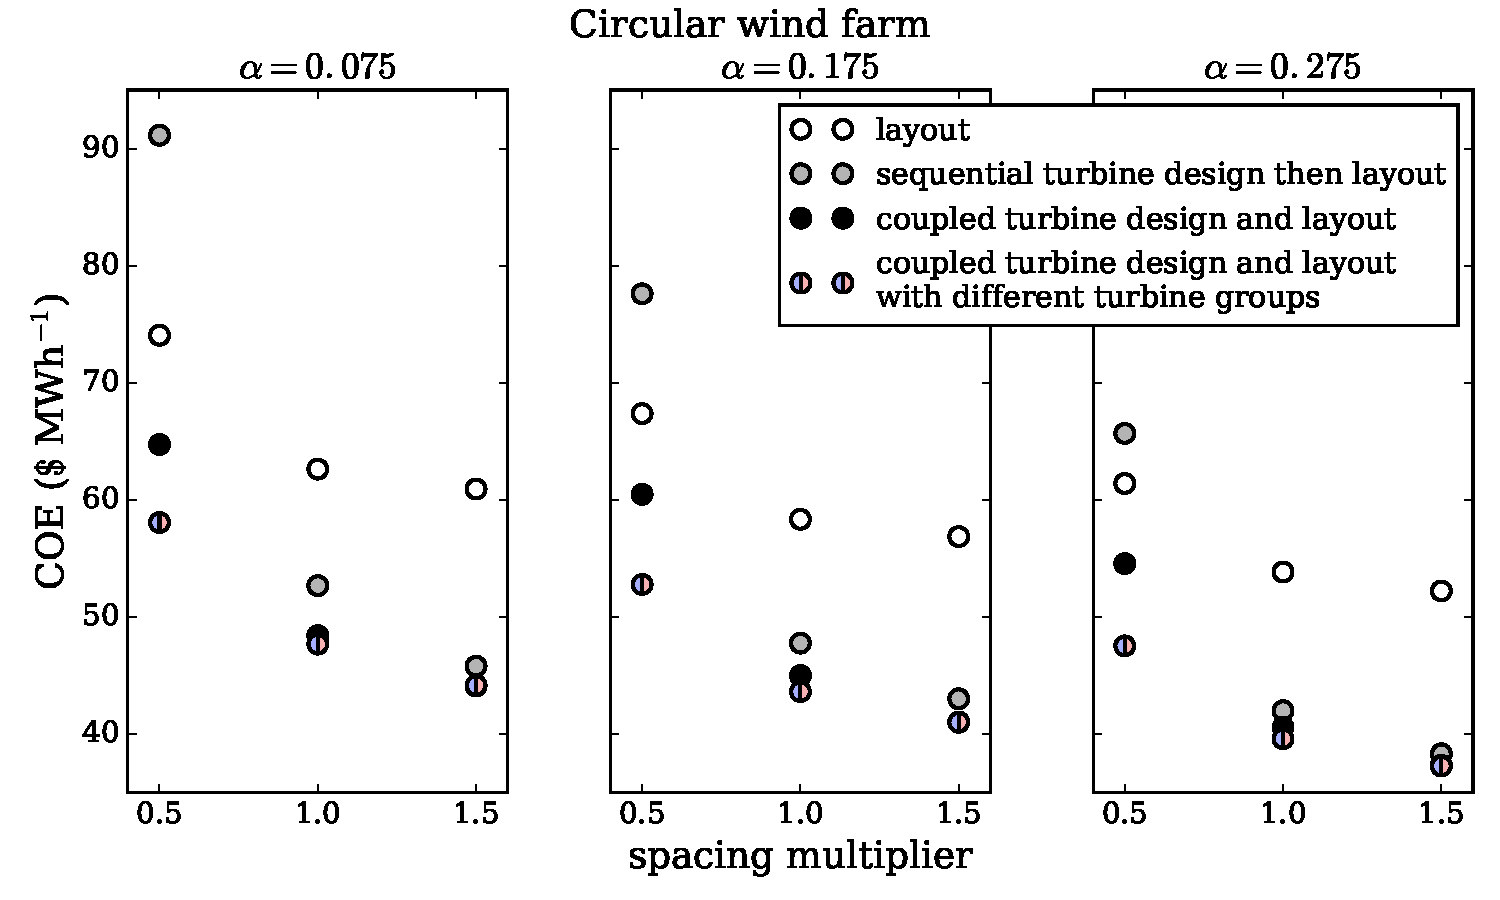
\includegraphics[width=0.8\textwidth]{Figures/circular_results1.pdf}
  \caption{\label{circular_results} The optimal COE results for the circular wind farm layout with 32 turbines. Each of the subfigures corresponds to optimization runs with a different shear exponent, from left to right $\alpha=0.075,0.175,0.275$. Within each subfigure, the x axis shows the size of the wind farm based on the spacing multiplier, from left to right $\beta=0.5,1.0,1.5$. The different points represent the layout optimization, sequential turbine-design-then-layout optimization, coupled layout-and-turbine-design optimization with homogeneous turbine design throughout the farm, and layout-and-turbine-design optimization with two different turbine design groups.}
\end{figure}

\subsubsection{Sequential Turbine Design then Layout Optimization}
The gray dots show the optimal COE results for a sequential optimization. First, a turbine was designed for minimal COE in isolation with the freestream wind conditions. This turbine design was then used in the wind farm where the layout was optimized. 
The rotor diameter was constrained such that the turbine spacing constraints would be satisfied in the baseline farm where the turbine would be installed. This was only applicable for the smallest wind farms, where $\beta=0.5$. 
For each shear exponent, the optimal turbine design was the maximum rotor diameter and turbine rating allowed by the optimizer.
%: 160 meters and 10 megawatts. 
%The optimal height increased with the shear exponent: 90 meters, 147 meters, and 155 meters for the shear exponents of 0.075, 0.175, and 0.275, respectively.
Figure \ref{circular_turbines_seq} shows the optimal isolated turbine designs for each shear exponent and spacing multiplier, as well as the baseline turbine design. Because these turbines are optimized in isolation, the designs for $\beta=1.0,1.5$ are the same. The only affect the spacing multiplier has on the design is a possible maximum rotor diameter (as in the case of $\beta=0.5$).
When these optimized turbine designs are used in each wind farm instead of the baseline turbine design, there is a large COE improvement for the spacing multipliers of $\beta=1.0, 1.5$. For $\beta=1.0$, COE decreases 15.9--22.0\% compared to an optimized wind farm with the baseline turbine design. For $\beta=1.5$ the COE decrease is even larger, 24.8--26.6\% across all shear exponents. 
%For the smallest wind farm, $\beta=0.5$, the turbine design optimized in isolation results in an infeasible farm layout. The rotor diameter is so large and the farm area so small that no layout is possible where the turbine spacing constraints are satisfied. However, even when the turbine spacing constraints were removed, this sequential turbine-design-then-layout optimization resulted in a worse COE for shear exponents of $\alpha=0.075,0.175$ compared to the layout-only optimization, and only a slightly better COE (2.3\%) for $\alpha=0.275$. 
For the smallest wind farm, $\beta=0.5$, the turbine design optimized in isolation results in an extremely inefficient wind farm. When in the wind farm environment, exposed to much lower average wind speeds, this design results in a COE that is much worse than the baseline turbine design. The expense from a bigger and taller turbine, coupled with the strong wake interactions among turbines that are so closely spaced means that for this wind farm, optimizing the turbine in isolation actually decreases the wind farm performance. 

\begin{figure}[htbp]
  \centering
  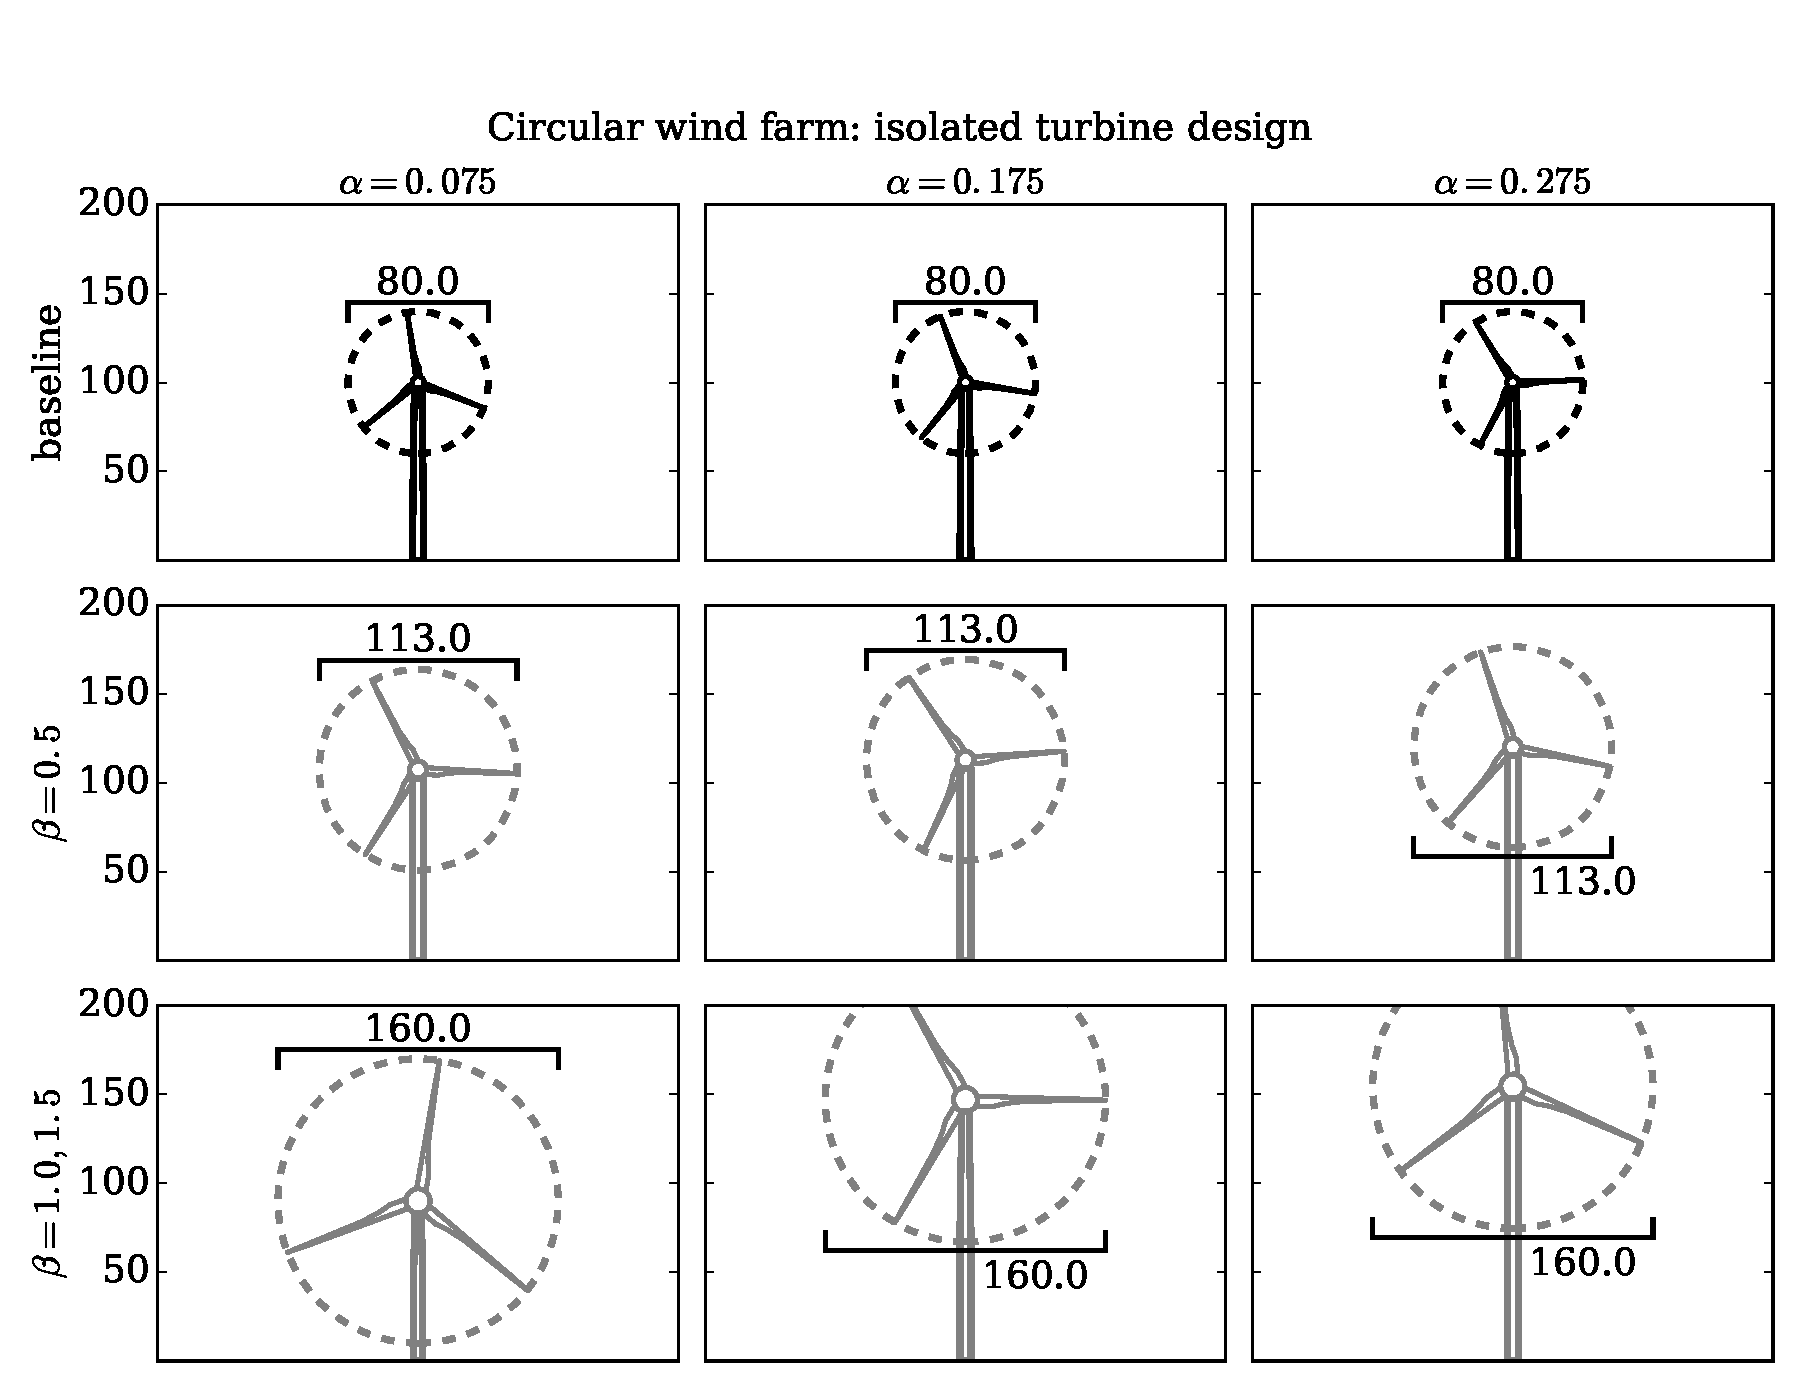
\includegraphics[width=0.8\textwidth]{Figures/turbineSizesCircular_sequential.pdf}
  \caption{\label{circular_turbines_seq} The optimal turbine heights and rotor diameters for the isolated turbine design optimization for the circular farm wind conditions. These designs were then used in the sequential turbine-design-then-layout optimizations. The columns, from left to right, show the turbines optimized for $\alpha=0.075,0.175$, and $0.275$. The rows, from top to bottom, show the baseline turbine design, the turbine optimized for the small wind farm ($\beta=0.5$), and the turbine designs for the larger wind farms ($\beta=1.0,1.5$)}
\end{figure}


\subsubsection{Coupled Turbine Design and Layout Optimization}
Next we will discuss the optimization results of the coupled turbine-design-and-layout optimizations, represented by the black dots in Fig. \ref{circular_results}. For every shear exponent and spacing multiplier, there is a large benefit to performing the coupled turbine-design-and-layout optimization compared to the layout-only optimization. Additionally, and more importantly, the coupled optimization results in appreciably lower COE than the sequential design-then-layout optimization. Obviously for a spacing multiplier of $\beta=0.5$, the coupled optimization is far superior to the sequential in that it results in a feasible wind farm. For the spacing multiplier of $\beta=1.0$, 
% which results in feasible wind farms for the sequential optimizations as well as the coupled optimizations, 
compared to the sequential optimizations, coupled optimization results in an additional 6.82\%, 4.75\%, and 2.65\% COE improvement from layout only optimization for shear exponents $\alpha=0.075, 0.175,$ and $0.275$, respectively. For the largest wind farm, $\beta=1.5$, the coupled optimization results in an additional 2.78\%, 3.50\%, and 1.88\% COE improvement compared to the sequential case. 

There are several conclusions we can make from both the sequential and coupled turbine design and layout optimizations. First, and most apparent, optimizing turbine design results in a much better wind farm than a farm in which the turbines are selected arbitrarily or a priori. Second, and more importantly, optimizing turbine design coupled with the turbine layout is significantly better than optimizing the turbine design for the freestream wind conditions alone. In a wind farm, turbines rarely experience the freestream wind conditions as they are often waked by the other turbines in the farm. Therefore, the optimal turbine design is based on on average slower wind speeds than the freestream wind. This results in turbines with smaller hub heights, rotor diameters, and rated powers. 

Figure \ref{circular_turbines_1} shows the optimal rotor diameters and hub heights for the coupled turbine design and layout optimizations. For a spacing multiplier $\beta=0.5$, the turbines are very close together and in general are heavily waked. Thus to satisfy spacing constraints and because the average wind speed is very low, the optimal rotor diameter is small: about 90 meters. When the turbines are spaced farther apart, shown for the larger spacing multipliers, the optimal rotor diameter is much larger: closer to 120--130 meters. In these farms, wake interactions are not as severe, meaning that the extra power production from larger rotors is worth the extra turbine capital cost. Also notice the trend of the optimal turbine height with wind shear exponent. For a low wind shear exponent, $\alpha=0.075$, the wind speed does not drastically change with height (see Fig. \ref{wp075}). Therefore, for this wind condition it is desireable to have short hub heights with a lower turbine capital cost. For the higher shear exponents, $\alpha=0.175,0.275$, the wind speed increases much more with height (See Figs. \ref{wp175} and \ref{wp275}). In these cases, for every spacing multiplier, the extra cost of building the taller turbines is made up for in the additional power produced from the high wind speeds. Note that a larger rotor diameter reduces the relative spacing between turbines in the farm, as the original spacing was based on a diameter of 80 meters.


\begin{figure}[htbp]
  \centering
  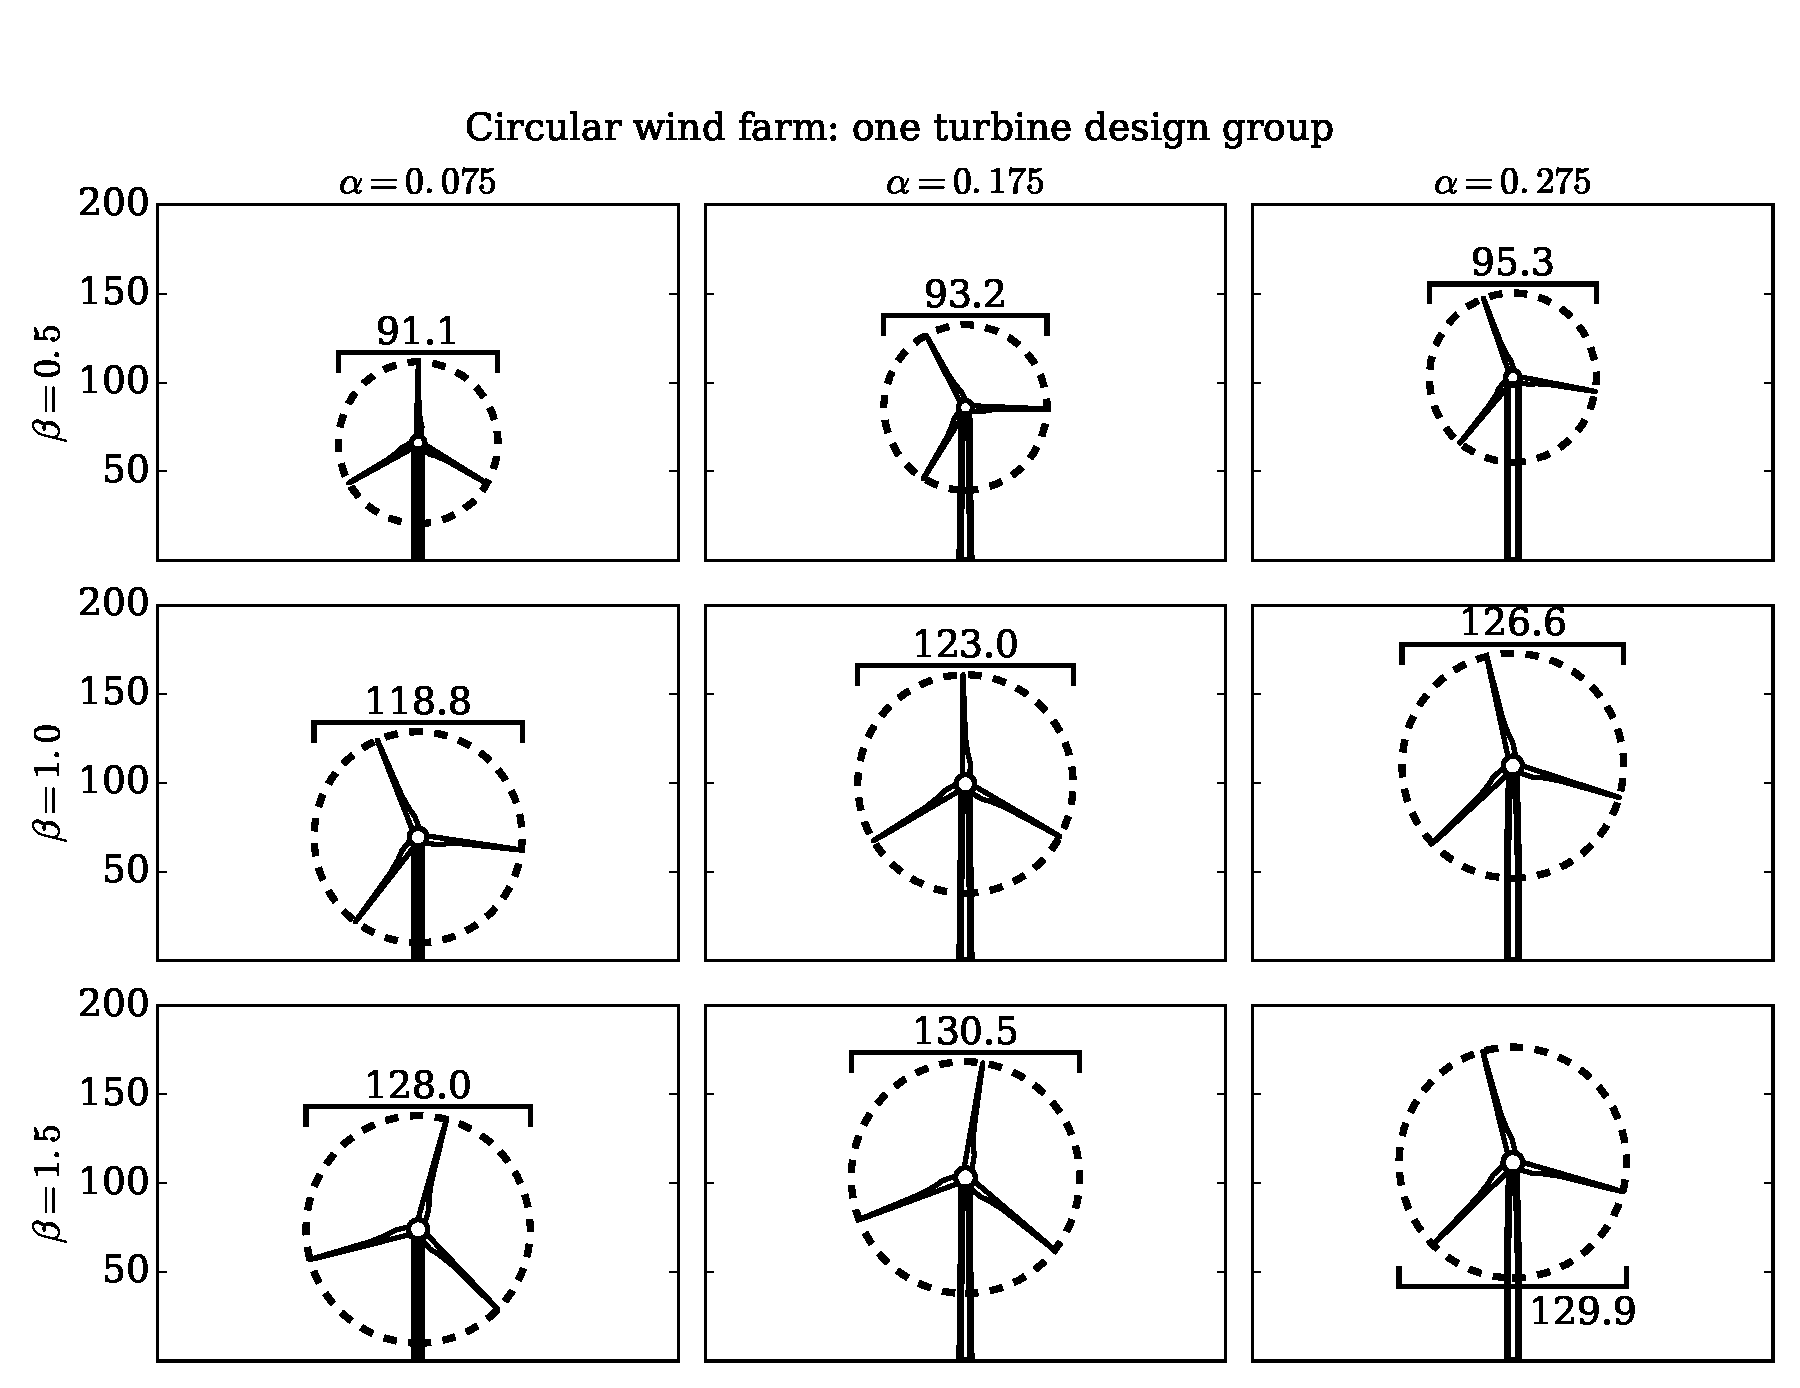
\includegraphics[trim={0.5cm 0.3cm 0.3cm 1.75cm},clip,width=0.8\textwidth]{Figures/turbineSizesCircular_1.pdf}
  \caption{\label{circular_turbines_1} The optimal turbine heights and rotor diameters for the optimization runs with coupled layout and turbine design with homogeneous turbine design throughout the circular wind farm. Each column shows a different shear exponent, with $\alpha=0.075,0.175,0.275$ from left to right. Each row shows a different farm spacing multiplier, with $\beta=0.5,1.0,1.5$ from top to bottom.}
\end{figure}

In Fig. \ref{circular_power}, the black points show the optimal rated powers for the turbines in each optimization case. Notice that the optimal rated power scales with the turbine rotor diameter and hub height. Higher turbine rating is expensive. Therefore, the small rotors and short turbines, which are more heavily waked and don't produce as much power, do not require a large power rating. The extra cost is not justified by a very slight increase in power. For the high shear exponents and spacing multipliers, the turbines are exposed to faster wind speeds. These turbines are bigger and taller, and the extra power production from raising the rated pwoer is worth the additional cost.



\subsubsection{Coupled Turbine Design and Layout Optimization with Two Turbine Groups}

Now we will discuss the most interesting case, the coupled turbine design and layout optimization with two different turbine groups. The optimal COE results of these optimziations are shown with the blue and pink points in Fig. \ref{circular_results}. Most visibly, for the smallest spacing multiplier, $\beta=0.5$, there is a large COE improvement for the hetergenous turbine design optimizations compared to the farms with homogeneous turbine design (shown by the black points in Fig. \ref{circular_results}). For this spacing multiplier, the heterogenous turbine design farms reduce COE by 21.6\%, 21.67\%, and 22.6\% compared to the layout-only optimization for shear exponents of $\alpha=0.075,0.175$, and $0.275$, respectively. The coupled optimizations with one turbine group reduce COE by 12.59\%, 10.24\%, and 11.15\%. For the smallest spacing multiplier, optimizing turbine design and layout with two turbine groups reduces COE by an additional 9--11.45\% compared to just one turbine group. For the spacing multiplier $\beta=1.0$, the coupled optimization with two turbine groups results in an additional 1.16--2.35\% COE decrease compared to with one turbine group. This is much smaller than the more tightly packed wind farms, but still non-negligible. For the spacing multiplier $\beta=1.5$, the optimization with two turbine groups results in only an additional 0--0.12\% COE decrease, indicating that when the turbines are spread very far apart there is no benefit to allowing multiple turbine designs in the same farm.

The two different rotor designs in the same wind farm help to improve COE by reducing the wake interaction between wind turbines. By combining tall and short turbines, with large and small rotor sizes, there are more dimensions that the optimizer can manipulate to avoid wakes and improve performance. For the tightly packed wind farms, the turbine layout is greatly limited by the turbine spacing constraints. Additionally, as the turbines are closer together, the wakes greatly reduce the wind speed as they have not had an opprtunity to mix with the freesteam air. Both of these factors mean there is a large benefit to avoiding the wakes of other turbines by any means possible. For the larger wind farms where the turbines are spaced farther apart, the wakes are not as detrimental and there is more area in which to avoid wakes in the horizontal plane without needing to change hub height or rotor diameter. In these cases, the heterogenous turbine designs are not as beneficial.

Figure \ref{circular_turbines} shows the optimal rotor diameter and hub height of each turbine group for these cases of coupled turbine design and layout optimization with two different groups. For the spacing multiplier $\beta=0.5$, when the turbines are very close together, there is a large difference in both the rotor diameter and hub height of each turbine group. Group 1 is extremely small and short, smaller than even the baseline rotor diameter, while Group 2 is much larger. Even if turbines from each group were right next to each other, there would be minimal wake interaction between the turbines. For the small wind farms, the sacrifice in power that comes from one very small and short turbine is made up for in the decreased wake inteference between turbine groups. Essentially, having two different turbine groups doubles the effective spacing between turbines, because turbines in different groups do not affect each other. For a larger spacing multiplier of $\beta=1.0$, each turbine group is still remarkably different in size and height. The turbines are larger than they were for the smallest wind farm because the average wind speed is faster when the turbines are spread farther apart. Notice that, compared to the optimized turbines for $\beta=0.5$, the smaller turbines when $\beta=1.0$ are larger and overlap more with the taller, bigger turbines. In this case, the power increase from bigger rotor diameters outweighs the benefit gained from reducing wake interference. 

The turbine sizes for the largest wind farm, $\beta=1.5$, demonstrate the multi-modality of the wind farm optimization problem. For this spacing multiplier, each turbine group is much more similar than in the previous wind farm sizes. For the lowest shear exponent, $\alpha=0.075$, both turbine groups are almost identical. For $\alpha=0.175,0.275$, there is some difference in each rotor diameter and hub height, although the difference is not as pronounced as it was for the smaller wind farms. However, Fig. \ref{circular_results} shows that for $\beta=1.5$ the optimal COE from coupled turbine design and layout optimization is the same with one and two height groups. So, a wind farm with the homogeneous turbine design shown in the bottom row of Fig. \ref{circular_turbines_1}, and a wind farm with two different turbine designs shown in the bottom row of Fig. \ref{circular_turbines} result in the same COE. The same optimal result is achieved with drastically different farms, each with different turbines and layouts.  

\begin{figure}[htbp]
  \centering
  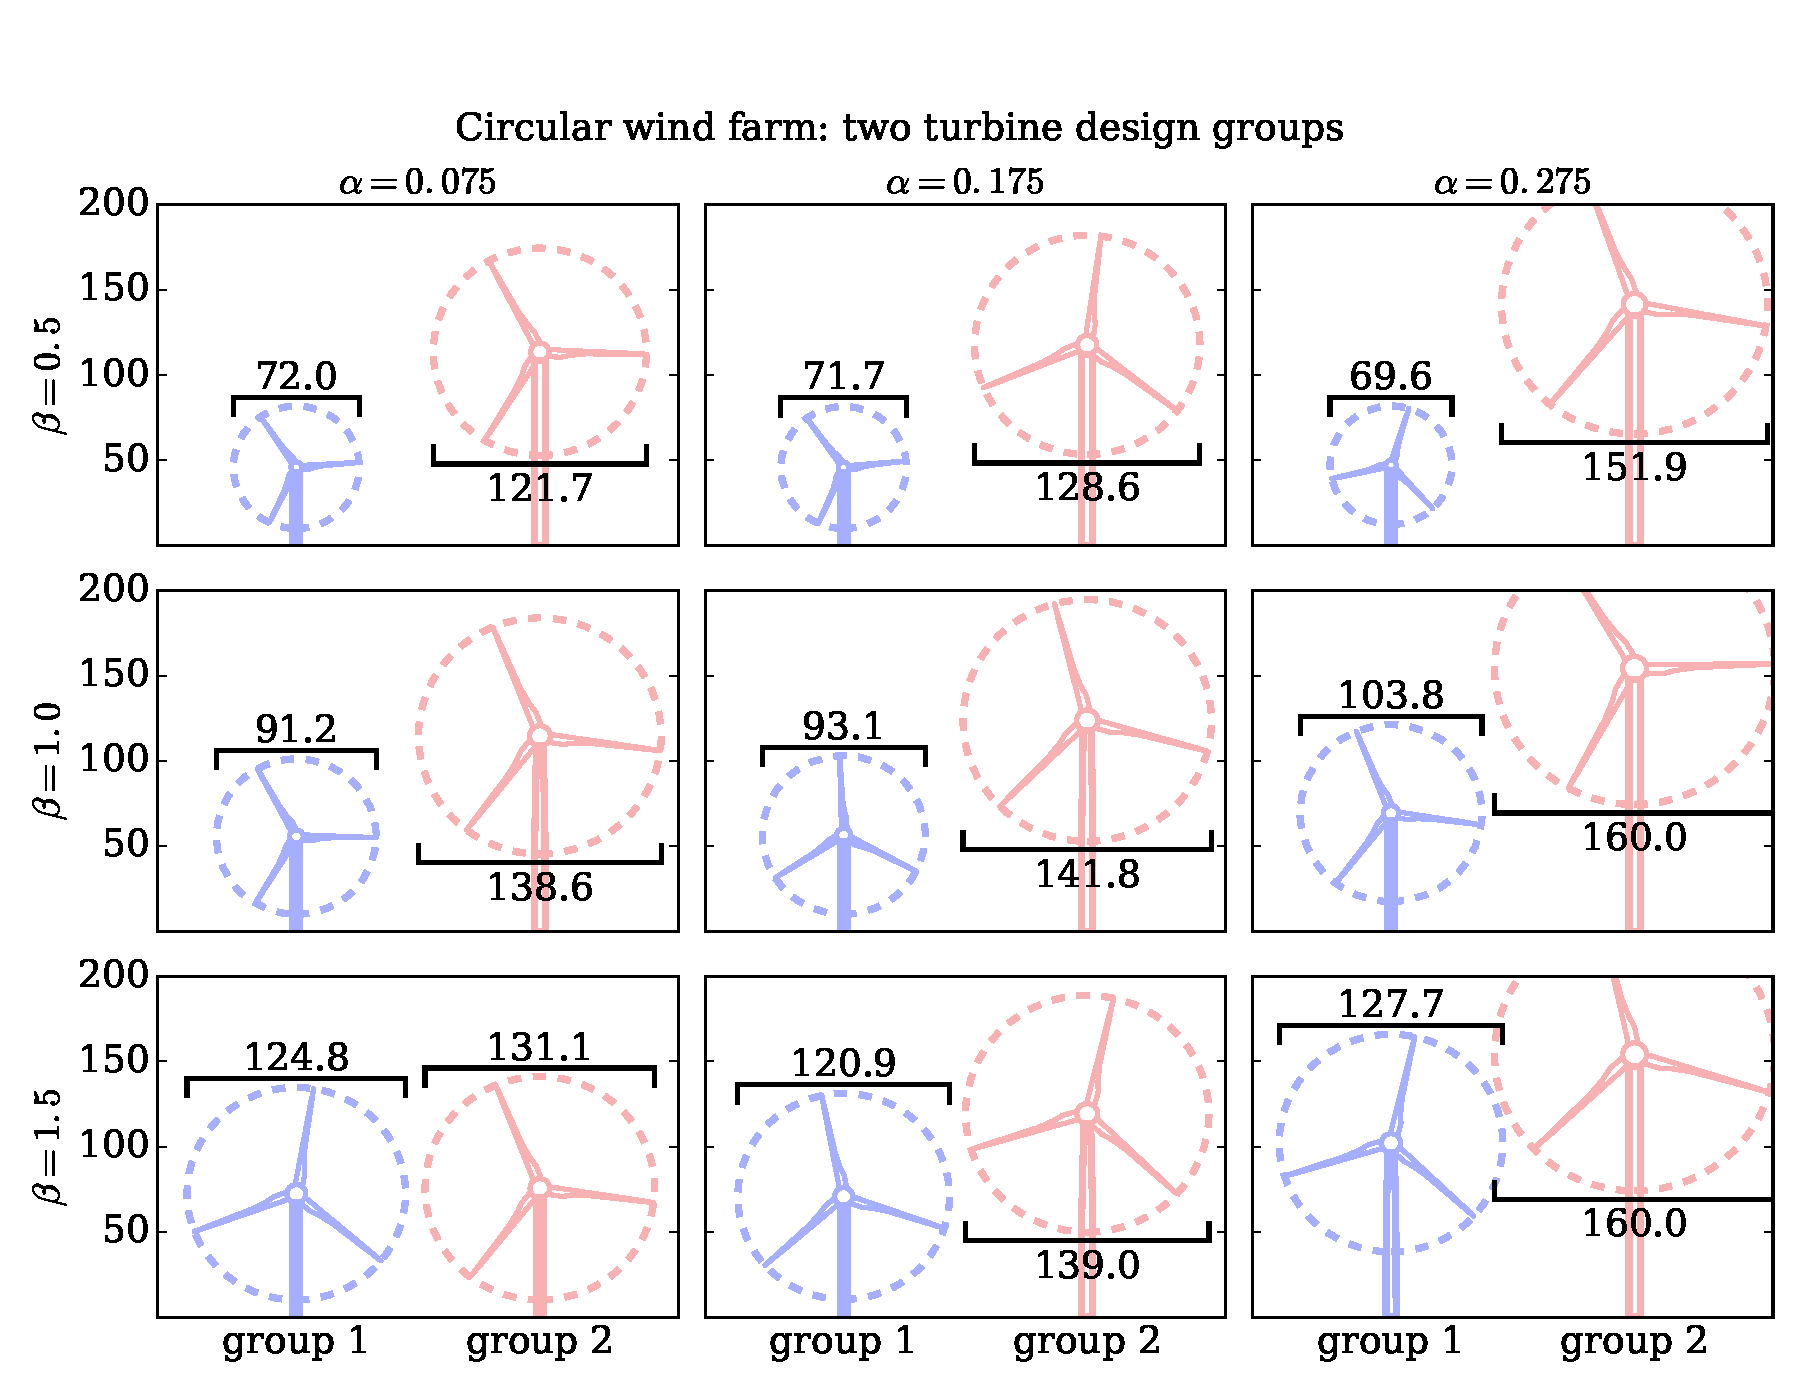
\includegraphics[trim={0.5cm 0.3cm 0.3cm 1.75cm},clip,width=0.8\textwidth]{Figures/turbineSizesCircular_2.pdf}
  \caption{\label{circular_turbines} The optimal turbine heights and rotor diameters for the optimization runs with coupled layout and turbine design with two different turbine design groups for the circular wind farm. Each column shows a different shear exponent, with $\alpha=0.075,0.175,0.275$ from left to right. Each row shows a different farm spacing multiplier, with $\beta=0.5,1.0,1.5$ from top to bottom.}
\end{figure}


Figure \ref{circular_power} shows the optimal rated power of each height group for the optimization cases with two different turbine groups. The blue and pink dots in this plot correspond to the turbines of the same color in Fig. \ref{circular_turbines}. As with the homogeneous turbine wind farm, the optimal rated power scales with the optimal turbine height and diameter. These larger, taller turbines are optimal in wind farms where they will be exposed to high wind speeds and produce large amounts of power. From a power production standpoint, it is undesirable to ever have a turbine's power limited by the rating. However, turbines with high ratings are more expensive, and not worth the cost if the turbine is generally producing low amounts of power. Therefore, the short, small turbines are optimal with a low, cheap power rating. The larger, taller turbines which produce much more electricity utilize the higher ratings. 


\begin{figure}[htbp]
  \centering
  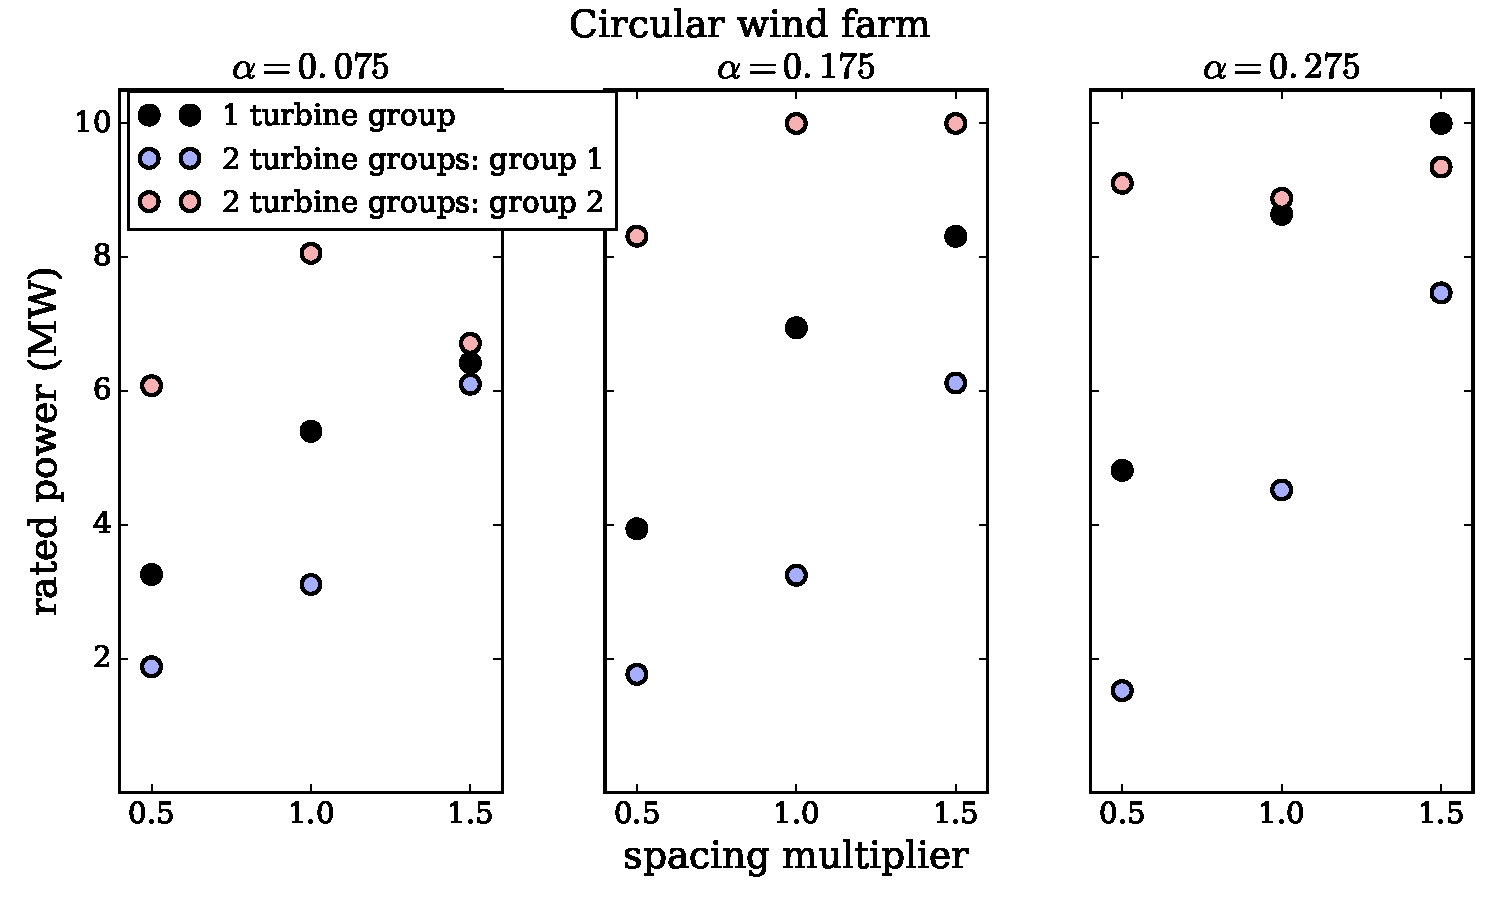
\includegraphics[width=0.8\textwidth]{Figures/circlePowers.pdf}
  \caption{\label{circular_power} The optimal rated powers for the circular wind farm for the optimization runs with coupled layout and turbine design for both uniform wind farm turbine design and with two different turbine design groups. The three subfigures show a different shear exponent, with $\alpha=0.075,0.175,0.275$ from left to right. within each subfigure, the x axis shows different farm spacing multipliers, with $\beta=0.5,1.0,1.5$ from left to right.}
\end{figure}

Table \ref{circular_table} shows how the optimal COE results shown in Fig. \ref{circular_results} compare to the layout optimization with the baseline wind turbine design. These numbers are to compare the relative benefit of performing turbine design with the various scenarios mentioned; they do not indicate a superior wind farm. Take for example two cases, Case A and Case B. Case A is when $\alpha=0.075$ and $\beta=0.5$, for the coupled turbine design and layout optimization with two turbine groups. This Case has an optimal COE 21.6\% lower than the layout-only optimization COE. For Case B, when $\alpha=0.275$ and $\beta=0.5$ for the coupled turbine design with just one height group, the optimal COE is 11.15\% lower than the layout-only optimization case. This does not mean that Case A is better than B (it is not, as seen in Fig. \ref{circular_results}); it simply means that it is able to a achieve a greater COE improvement relative to the layout optimization baseline case. With this in mind, notice that for a spacing multiplier $\beta=0.5$, the relative improvement of two turbine design groups is far superior to coupled design and layout optimization with one turbine group. Also, for $\beta=0.5,1.0$, coupled turbine design and layout optimization is significantly better than the sequential optimization.

\begin{center}
\begin{table}
\caption{The percent COE decrease of the various optimization cases with respect to layout-only optimization performed for the circular wind farm. This table does not show the overall desirability of the optimal wind farm, but the relative improvement of different considerations of turbine design optimization. In the table are shown results for each shear exponent, $\alpha$, as well as each spacing multiplier, $\beta$, in which the smaller spacing multipliers represent farms with turbines that are more closely spaced.}
\label{circular_table}
\begin{tabular}{p{2.5cm} c c c c c c c c c c c}
%\begin{tabularx}{\textwidth}{|X|c|c|c|c|c|c|c|c|c|}
\hline
\multicolumn{10}{c}{\textbf{circular wind farm: percent COE decrease from layout only optimization}}\\
\hline
 & \multicolumn{3}{c}{$\alpha=0.075$} & \multicolumn{4}{c}{$\alpha=0.175$} & \multicolumn{4}{c}{$\alpha=0.275$}\\
\hline
optimization case & $\beta\myeq0.5$ & $\beta\myeq1.0$ & $\beta\myeq1.5$ & & $\beta\myeq0.5$ & $\beta\myeq1.0$ & $\beta\myeq1.5$& &$\beta\myeq0.5$ & $\beta\myeq1.0$ & $\beta\myeq1.5$\\
%\specialrule{.2em}{.1em}{.1em}
sequential & \textcolor{red}{-23.07} & 15.90 & 24.84 & & \textcolor{red}{-15.19}  & 18.13 & 24.37 & & \textcolor{red}{-6.97}  & 22.01 & 26.64\\
%\hline
coupled: 1 group& 12.59  & 22.72  & 27.62  & & 10.24  & 22.88  & 27.87 & & 11.15 & 24.66 & 28.52 \\
%\hline
coupled: 2 groups & 21.60  & 23.88  & 27.54 & & 21.67  & 25.23  &  27.90 & &  22.60 & 26.46  & 28.64\\
\hline
%\end{tabularx}
\end{tabular}
\end{table}
\end{center}











\subsection{Princess Amalia Wind Farm Results}

Figure \ref{amalia_results} shows the COE results for the 60-turbine Princess Amalia wind farm optimizations.  The trends are similar to the smaller, circular wind farm. Coupled turbine design and layout optimization is superior to optimizing each sequentially, especially for the smaller wind farms where the wind speeds are much lower than the free stream. For the farms with closely spaced wind turbines, two different turbine designs in the same farm are significantly better than the farms optimized with a homogeneous turbine design. If the largest wind farms ($\beta=1.5$) benefit from two different turbine design groups, that benefit is negligible. 

\begin{figure}[htbp]
  \centering
  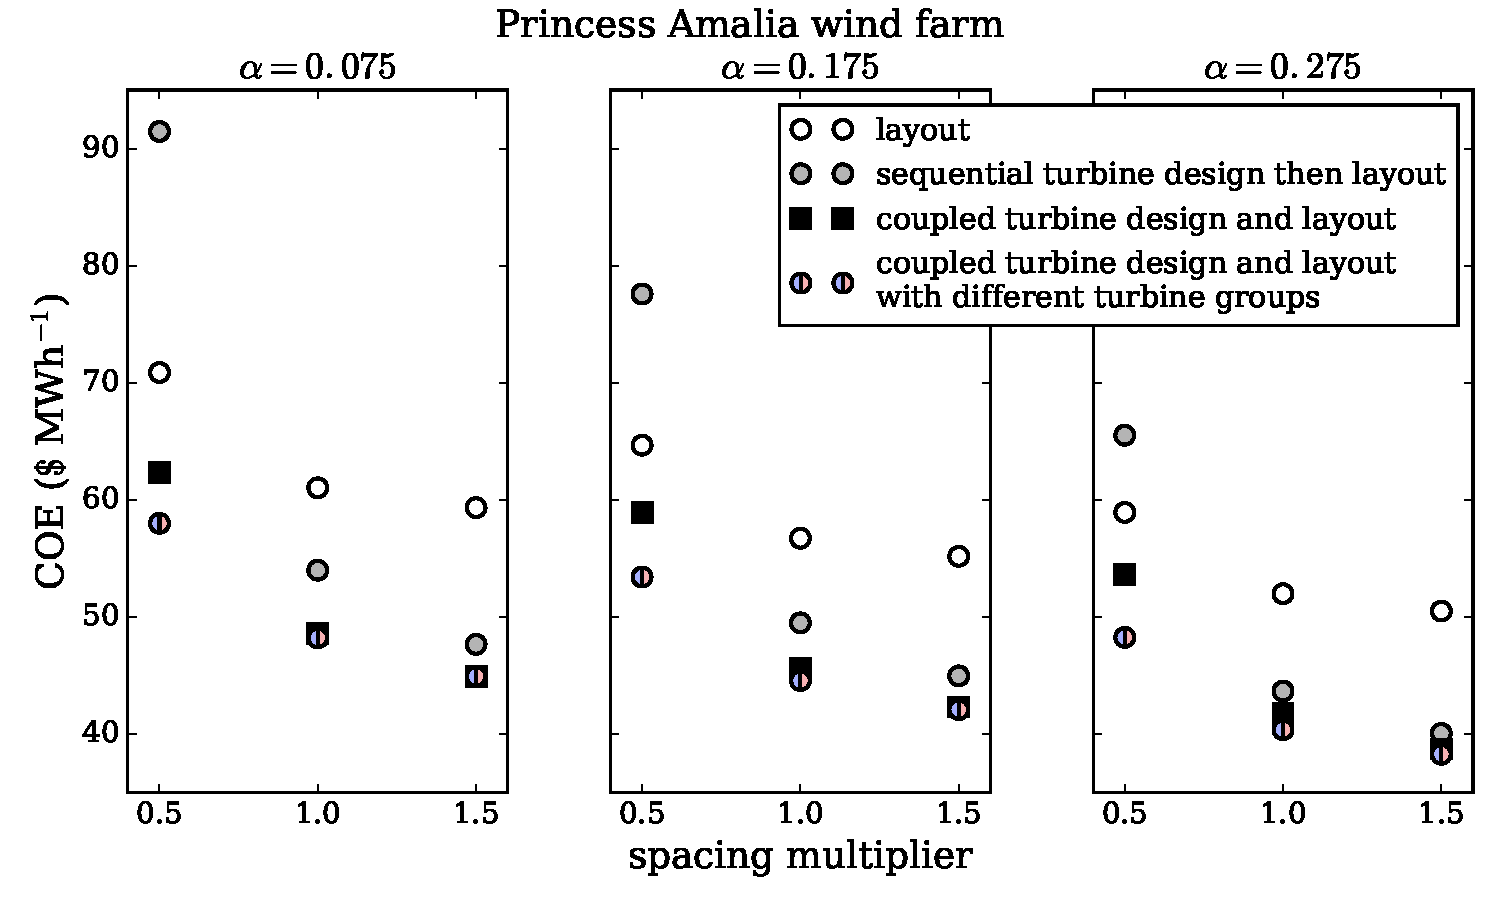
\includegraphics[width=0.8\textwidth]{Figures/amalia_results1.pdf}
  \caption{\label{amalia_results} The optimal COE results for the Princess Amalia wind farm layout with 32 turbines. Each of the subfigures corresponds to optimization runs with a different shear exponent, from left to right $\alpha=0.075,0.175,0.275$. Within each subfigure, the x axis shows the size of the wind farm based on the spacing multiplier, from left to right $\beta=0.5,1.0,1.5$. The different points represent the layout optimization, sequential turbine-design-then-layout optimization, coupled layout-and-turbine-design optimization with homogeneous turbine design throughout the farm, and layout-and-turbine-design optimization with two different turbine design groups.}
\end{figure}

Figures \ref{amalia_turbines_seq}, \ref{amalia_turbines_1},  and \ref{amalia_turbines} show the turbine rotor diameters and hub heights for the various optimization runs,  Fig. \ref{amalia_power} shows the optimal rated powers for the coupled turbine-design-and-layout optimizations, and Table \ref{amalia_table} tabulates the relative benefit of each optimization compared to the layout only optimization. The trends, and reasons behind them, are the same as for the circular wind farm optimizations. We will therefore not repeat this discussion, but will briefly discuss the significant differences between the optimizations of the 32-turbine circular wind farm and those for the 60-turbine Princess Amalia wind farm. The optimal COE values for the Princess Amalia wind farm are slightly lower across the board than the circular wind farm COE values. This is partly because there are more turbines in the Princess Amalia wind farm so a smaller portion of the total cost comes from overhead, but is partly due to the Princess Amalia wind turbines being spaced slightly farther apart than those in the circular wind farms. Another major difference between the optimal COE values of each wind farm is in the optimization case with two turbine design groups. For the Princess Amalia wind farm and a spacing multiplier of 0.5, two turbine groups provides and additional COE decrease of 6.13--9.11\% compared to the wind farm with homogeneous turbine design. This is significant, however it is not as large as the 9.01--11.45\% additional COE decrease in the circular wind farm optimizations for the same spacing multiplier. Again, the main cause of this seems to be that the circular wind farms are slightly closer together than the Princess Amalia wind farms. The conclusion remains the same, wind farms with closely spaced wind turbines greatly benefit from different turbine designs. The last significant difference between the wind farm is that the optimal turbine designs for the Princess Amalia wind farms are slightly smaller than in the circular wind farms. This is due to the different wind roses and speed distributions used to optimized each wind farm. 







%\subsubsection{Sequential Turbine Design then Layout Optimization}

\begin{figure}[htbp]
  \centering
  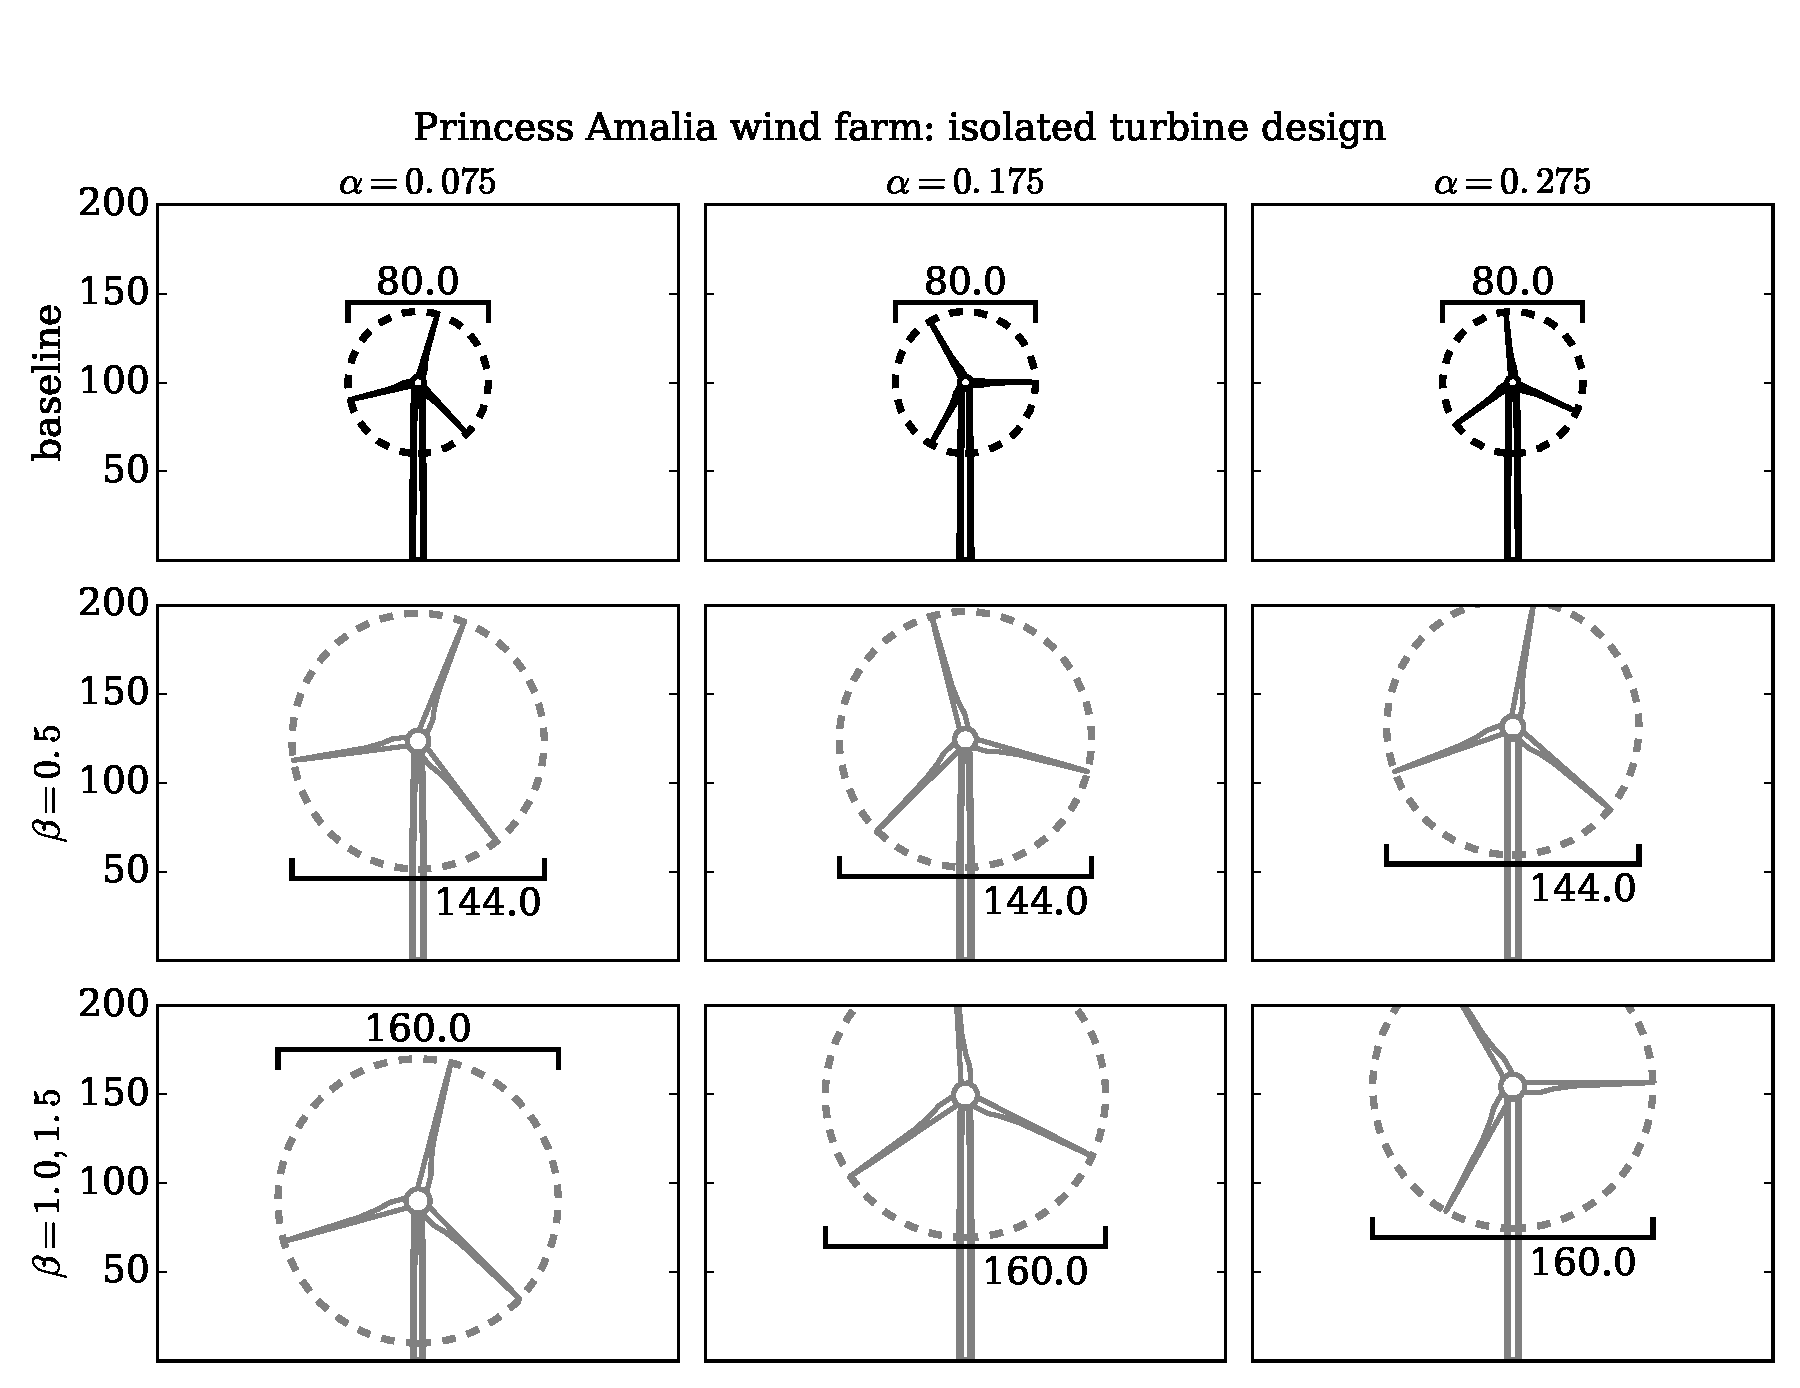
\includegraphics[width=0.8\textwidth]{Figures/turbineSizesAmalia_sequential.pdf}
  \caption{\label{amalia_turbines_seq} The optimal turbine heights and rotor diameters for the isolated turbine design optimization for the Princess Amalia farm wind conditions. These designs were then used in the sequential turbine-design-then-layout optimizations. The columns, from left to right, show the turbines optimized for $\alpha=0.075,0.175$, and $0.275$. The rows, from top to bottom, show the baseline turbine design, the turbine optimized for the small wind farm ($\beta=0.5$), and the turbine designs for the larger wind farms ($\beta=1.0,1.5$)}
\end{figure}




%\subsubsection{Coupled Turbine Design and Layout Optimization}

\begin{figure}[htbp]
  \centering
  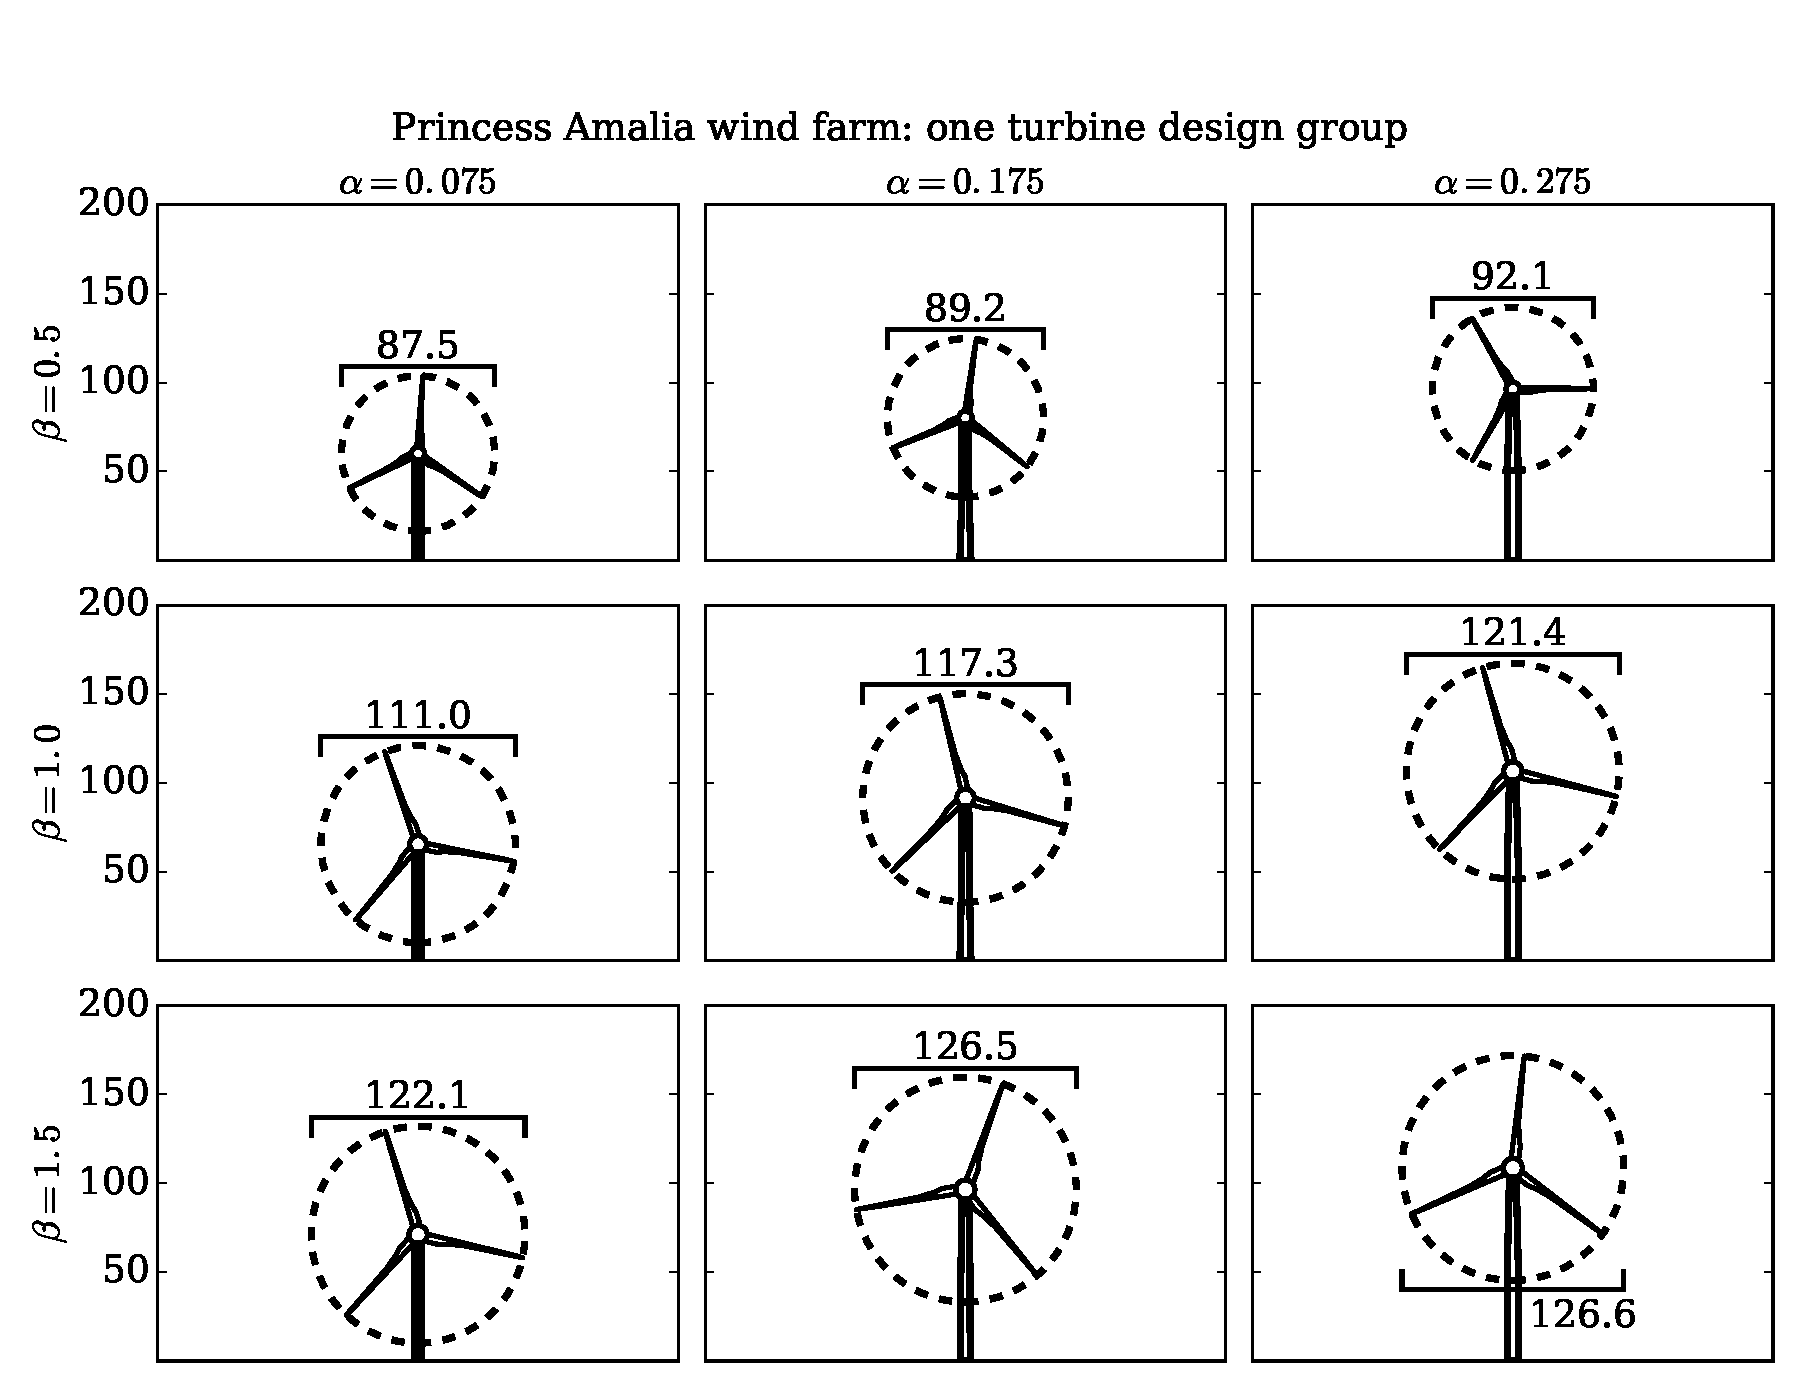
\includegraphics[trim={0.5cm 0.3cm 0.3cm 1.75cm},clip,width=0.8\textwidth]{Figures/turbineSizesAmalia_1.pdf}
  \caption{\label{amalia_turbines_1} The optimal turbine heights and rotor diameters for the optimization runs with coupled layout and turbine design with homogeneous turbine design throughout the circular wind farm. Each column shows a different shear exponent, with $\alpha=0.075,0.175,0.275$ from left to right. Each row shows a different farm spacing multiplier, with $\beta=0.5,1.0,1.5$ from top to bottom.}
\end{figure}



%\subsubsection{Coupled Turbine Design and Layout Optimization with Two Turbine Groups}

\begin{figure}[htbp]
  \centering
  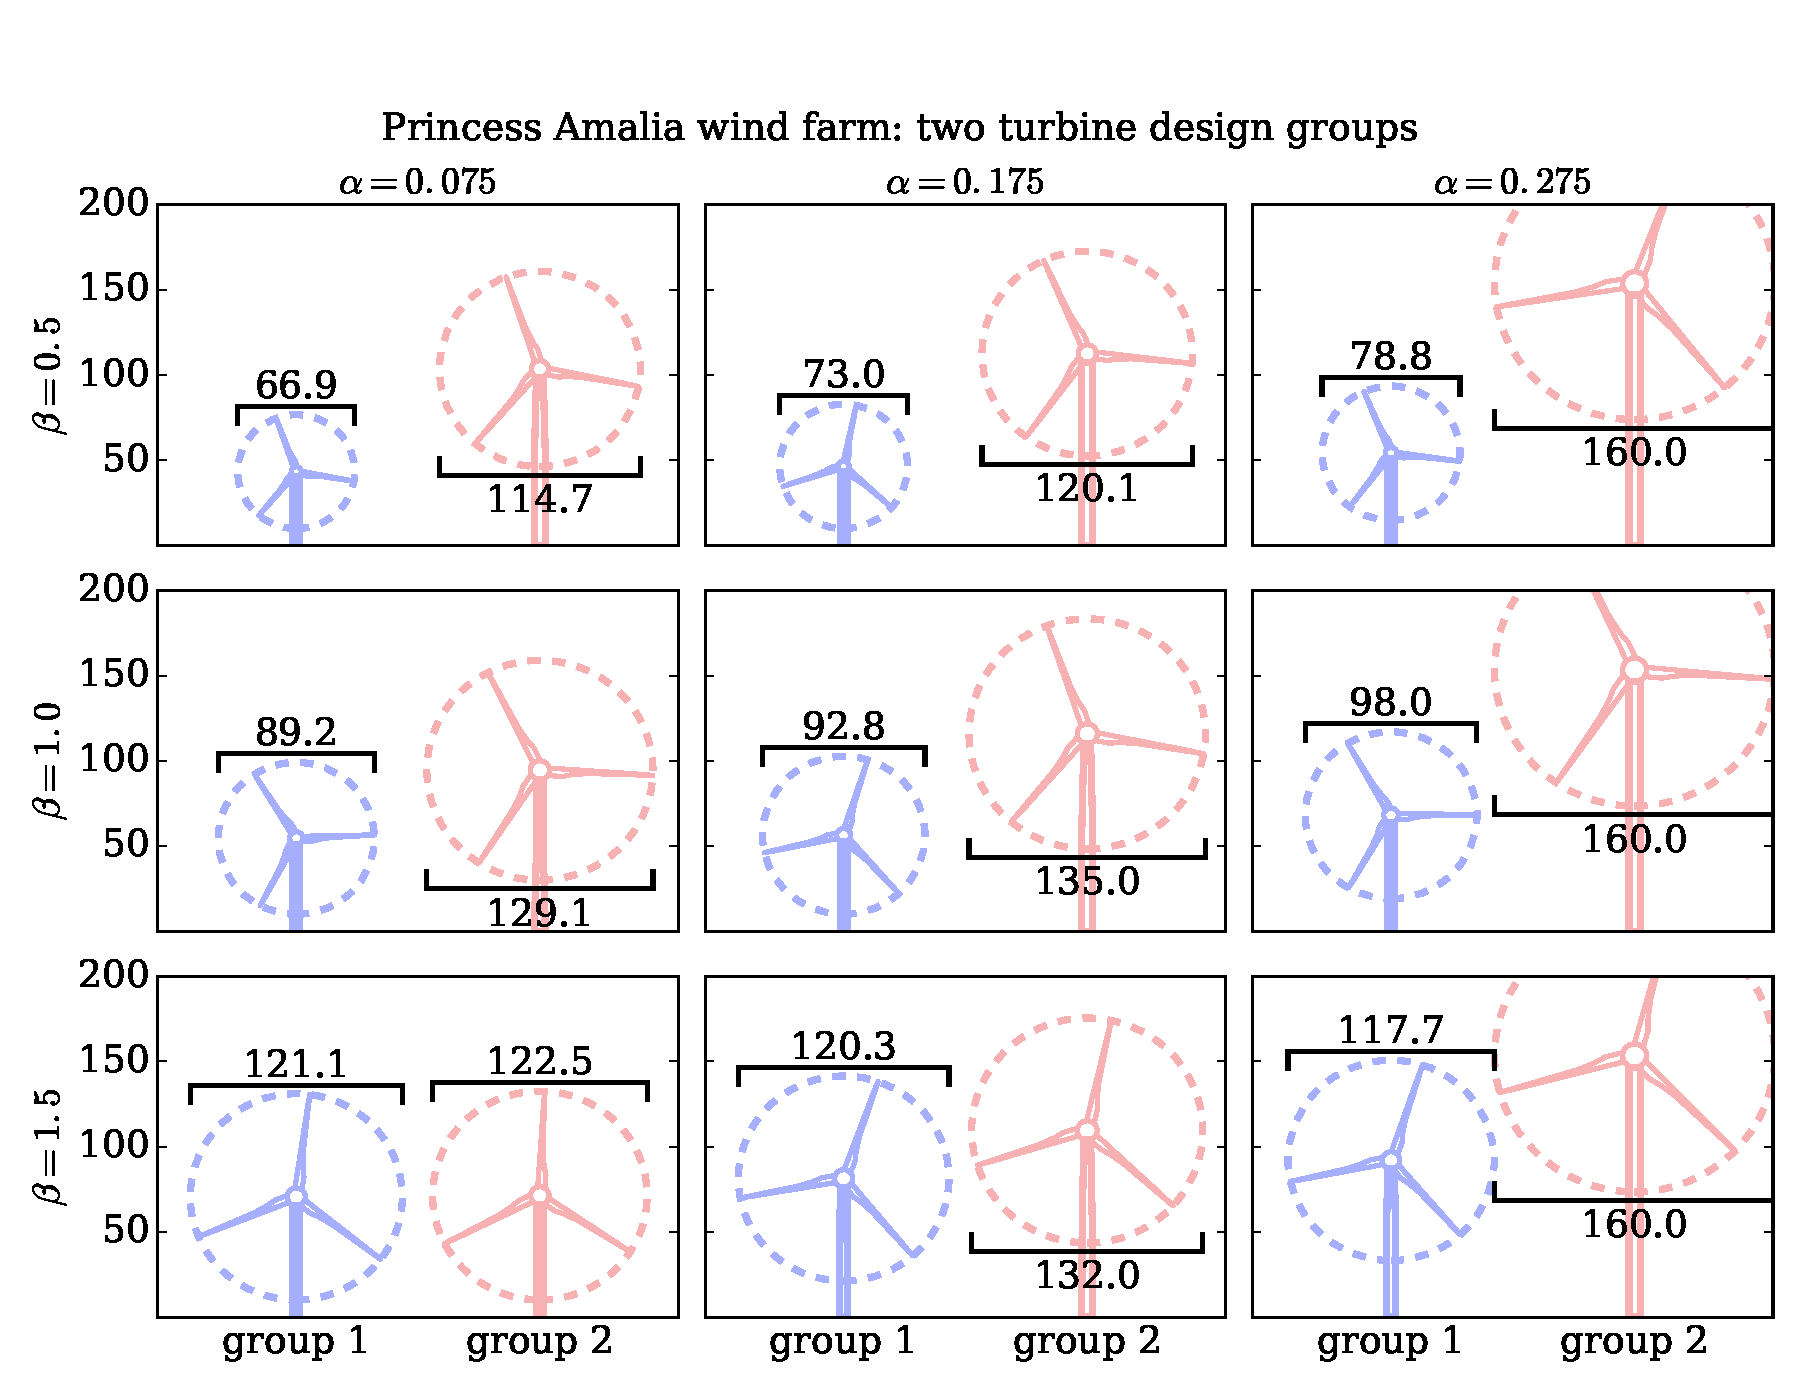
\includegraphics[trim={0.5cm 0.3cm 0.3cm 1.75cm},clip,width=0.8\textwidth]{Figures/turbineSizesAmalia_2.pdf}
  \caption{\label{amalia_turbines} The optimal turbine heights and rotor diameters for the optimization runs with coupled layout and turbine design with two different turbine design groups for the circular wind farm. Each column shows a different shear exponent, with $\alpha=0.075,0.175,0.275$ from left to right. Each row shows a different farm spacing multiplier, with $\beta=0.5,1.0,1.5$ from top to bottom.}
\end{figure}


\begin{figure}[htbp]
  \centering
  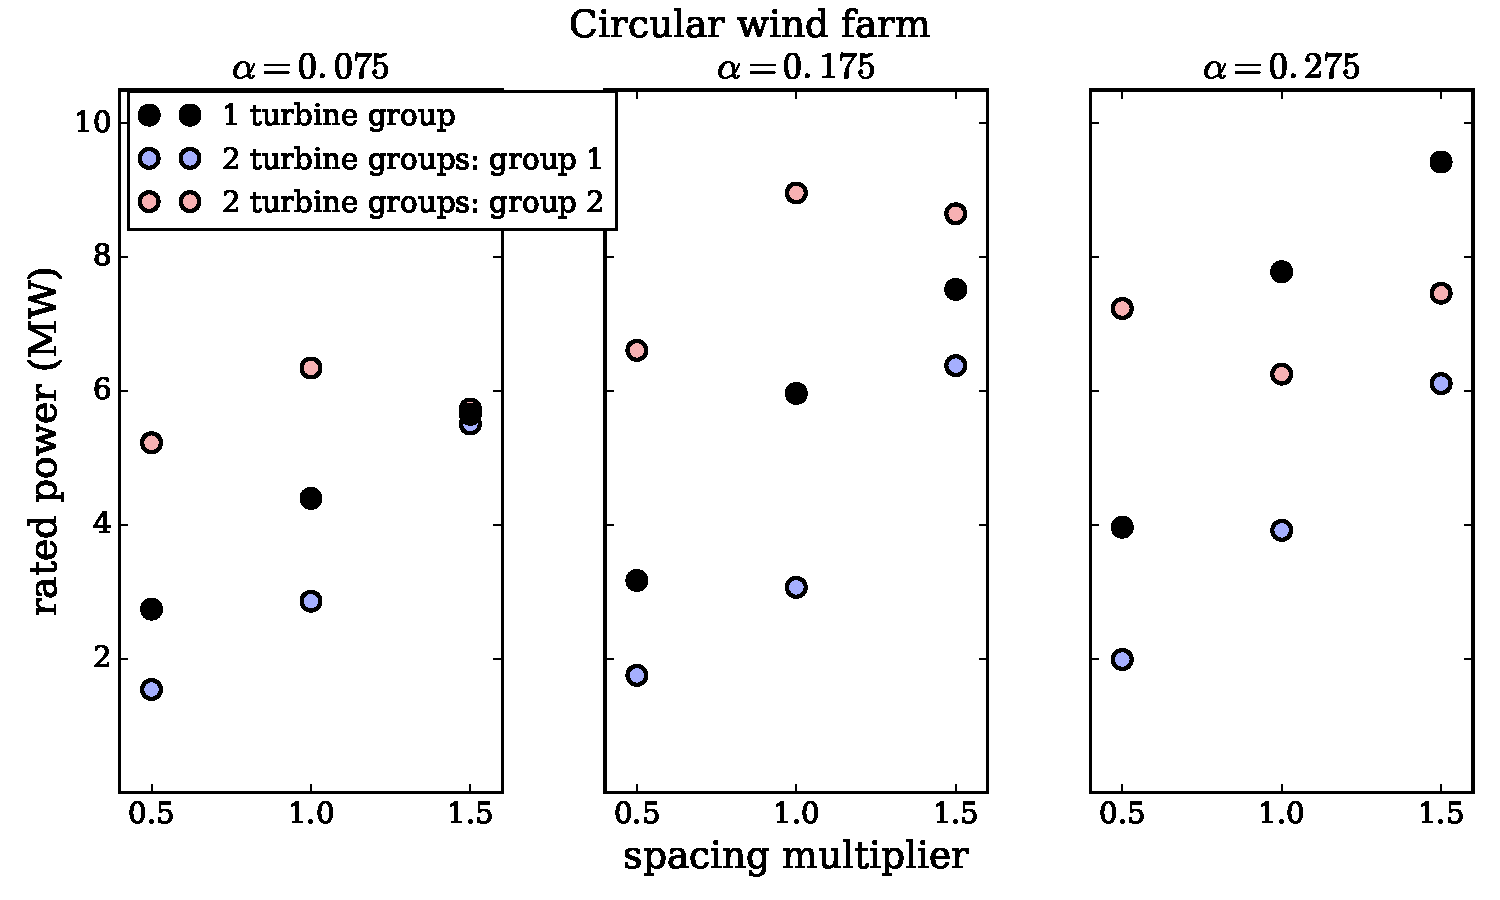
\includegraphics[width=0.8\textwidth]{Figures/amaliaPowers.pdf}
  \caption{\label{amalia_power} The optimal rated powers for the Princess Amalia wind farm for the optimization runs with coupled layout and turbine design for both uniform wind farm turbine design and with two different turbine design groups. The three subfigures show a different shear exponent, with $\alpha=0.075,0.175,0.275$ from left to right. within each subfigure, the x axis shows different farm spacing multipliers, with $\beta=0.5,1.0,1.5$ from left to right.}
\end{figure}




\begin{center}
\begin{table}
\caption{The percent COE decrease of the various optimization cases with respect to layout-only optimization performed for the Princess Amalia wind farm. This table does not show the overall desirability of the optimal wind farm, but the relative improvement of different considerations of turbine design optimization. In the table are shown results for each shear exponent, $\alpha$, as well as each spacing multiplier, $\beta$, in which the smaller spacing multipliers represent farms with turbines that are more closely spaced.}
\label{amalia_table}
\begin{tabular}{p{2.5cm} c c c c c c c c c c c}
%\begin{tabularx}{\textwidth}{|X|c|c|c|c|c|c|c|c|c|}
\hline
\multicolumn{10}{c}{\textbf{Princess Amalia wind farm: percent COE decrease from layout only optimization}}\\
\hline
 & \multicolumn{3}{c}{$\alpha=0.075$} & \multicolumn{4}{c}{$\alpha=0.175$} & \multicolumn{4}{c}{$\alpha=0.275$}\\
\hline
optimization case & $\beta\myeq0.5$ & $\beta\myeq1.0$ & $\beta\myeq1.5$ & & $\beta\myeq0.5$ & $\beta\myeq1.0$ & $\beta\myeq1.5$& &$\beta\myeq0.5$ & $\beta\myeq1.0$ & $\beta\myeq1.5$\\
%\specialrule{.2em}{.1em}{.1em}
sequential & \textcolor{red}{-29.06} & 11.54 & 19.70 & & \textcolor{red}{-19.98}  & 12.74 & 18.52 & & \textcolor{red}{-11.19}  & 16.02 & 20.70\\
%\hline
coupled: 1 group& 12.05  & 20.45  & 24.34  & & 8.94  & 19.61  & 23.32 & & 9.00 & 19.66 & 23.33 \\
%\hline
coupled: 2 groups & 18.18  & 21.01  & 24.30 & & 17.41  & 21.45  &  23.74 & &  18.11 & 22.37  & 24.24\\
\hline
%\end{tabularx}
\end{tabular}
\end{table}
\end{center}


% \subsection{Princess Amalia Wind Farm Optimization}

% % Figure \ref{amalia_results} shows the optimal COE results for the Princess Amalia wind farm. As expected, the higher wind speed from high wind shear results in a lower optimal COE. Additionally, the widely spaced wind turbines indicated by the larger spacing multipliers also result in lower COE. 
% % For every shear exponent and spacing multiplier there is a small decrease in optimal COE from the baseline wind farm to when layout optimization has occurred. The largest benefit from layout optimization occurs for the smallest wind farms with COE decreases from 2.39-2.48\%, while for spacing multiplier of 1.0 and 1.5, the COE decrease is negligible, from 0.26-0.62\%. In these cases where turbines are farther apart, there is already minimal wake interference between wind turbines, so layout optimization does not provide a significant benefit. The very small COE decrease, even for the spacing multiplier of 0.5, indicates that the baseline layout is already very good and that this is a well designed wind farm layout for the turbines that are used. 

% % Optimizing the turbine design along with the farm layout provides significant COE decrease compared to baseline, and compared to the layout only optimization. First we will discuss the turbine design optimization in which there is homogeneous design for all turbines in the wind farm. For a spacing multiplier of 0.5, there is a COE decrease of 11.24-14.46\% across all of the wind shears. For the more widely spaced wind farms, the COE decrease is even greater at 20.19-24.97\%. 
% % %
% % This is incredible! An additional 10-25\% decrease in COE from a wind farm with quasi-optimal turbine layout is amazing. Designing the wind turbines appropriately wind conditions they will experience in the wind farm environment can amount to worthwhile gains in energy production and cost reduction.
% % %
% % For the optimization cases that we ran, the larger wind farms benefited more from turbine design optimization than the smaller farm. For the larger wind farms, turbine wake interactions are not as detrimental because the slow moving wakes have begun to recover much of the momentum that was lost. Therefore, a turbine design with a large rotor and high rated power is cost effective. For the smaller wind farm, where the average wind speed is lower throughout the farm because of turbine wakes, a smaller turbine and lower rated power, closer to the original baseline values, is optimal.
% % %
% % % These results indicate the importance of designing turbines for the wind conditions and the specific wind farm where they will operate. Not only are the freestream wind conditions important, but the atmospheric boundary layer and the turbine spacing in the wind farm. Optimizing turbine design finds the hub height, rotor diameter, and rated power that best captures the energy in the wind farm for the lowest cost.

% % Now we will discuss the additional benefit that comes from two different turbine designs used throughout the wind farm. For the tightly spaced wind farms (spacing multiplier of 0.5), there is additional COE decrease in the wind farms with two different turbine groups. Across all the shear exponents, there is an additional 5.95-8.68\% COE decrease from baseline compared to the farm with homogeneous turbine design. In these tightly packed wind farms, there is significant wake interaction between the turbines. In such cases, having different turbine designs reduces the wake interaction with different hub heights and rotor diameters, as shown in the top row of Figure \ref{amalia_turbines}. For the spacing multiplier of 0.5, one turbine group is very short and small, while the other is taller and large. Rather than have all the turbines have a large swept area and be tall to reach the fast moving freestream air, it is more beneficial to have one small turbine group which avoids the wakes of the tall turbines, and doesn't produce wakes that will interfere much with the taller group. 
% % When the turbines are close to each other as they are with a spacing multiplier of 0.5, a lot of power is lost through wake interactions among turbines. Because of the tight spacing, moving turbines in the horizontal plane through layout optimization is not as successful in avoiding the wakes of other turbines. Thus in this case, the different heights and rotor diameters are very successful in reducing COE in a wind farm because they allow turbines to avoid wakes vertically as well as in the horizontal plane. 
% % The turbine rating of each group is also optimized to produce as much energy as each group is capable, but not be over-rated such that turbine costs rise without an associated increase in energy production. In the larger wind farms, there is still a small benefit to having the two different turbine groups, but not nearly as pronounced as the small wind farm. In the middle and bottom rows of Figure \ref{amalia_turbines} are the optimal sizes of the different turbine groups. The difference between the rotor diameters of each turbine group decreases as the distance between the turbines increases. For the largest spacing multiplier, the turbines in each group are almost exactly the same. When the turbines are farther apart, the wake interactions are not as detrimental, making it more beneficial to have the turbine groups be more similar to each other, and to the wind farm optimized with homogeneous turbine design.


% % Figure \ref{amalia_power} shows the optimal rated powers of each turbine group for each optimization. Note that the larger rated powers correspond to the taller, larger wind turbines from Figure \ref{amalia_turbines}. There is no need for the smaller and shorter turbines to have a very high rated power if the energy they can produce is limited by their size.
% % Table \ref{tab:amalia} shows the percent decrease in COE for each optimization case compared to the baseline. Note that the higher percent decrease does not mean a more desirable wind farm. The lowest overall COE is achieved in wind farms with a high wind shear and turbines spaced far apart. This table shows how much better a wind farm can be with turbine design and layout optimization, compared to a sub-optimal wind farm.


% % Figures \ref{amalia_turbines} and \ref{amalia_power} show the optimal turbine hub heights, rotor diameters, and rated powers for the wind farms with two different turbine groups. For the spacing multiplier of 0.5, there is a large difference between the hub heights and rotor diameters of each turbine group. When the turbines are close to each other as they are with a spacing multiplier of 0.5, a lot of power is lost through wake interactions among turbines. Because of the tight spacing, moving turbines in the horizontal plane through layout optimization is not as successful in avoiding the wakes of other turbines. Thus in this case, the different heights and rotor diameters are very successful in reducing COE in a wind farm because they allow turbines to avoid wakes vertically as well as in the horizontal plane. 


% \begin{figure}[htbp]
%   \centering
%   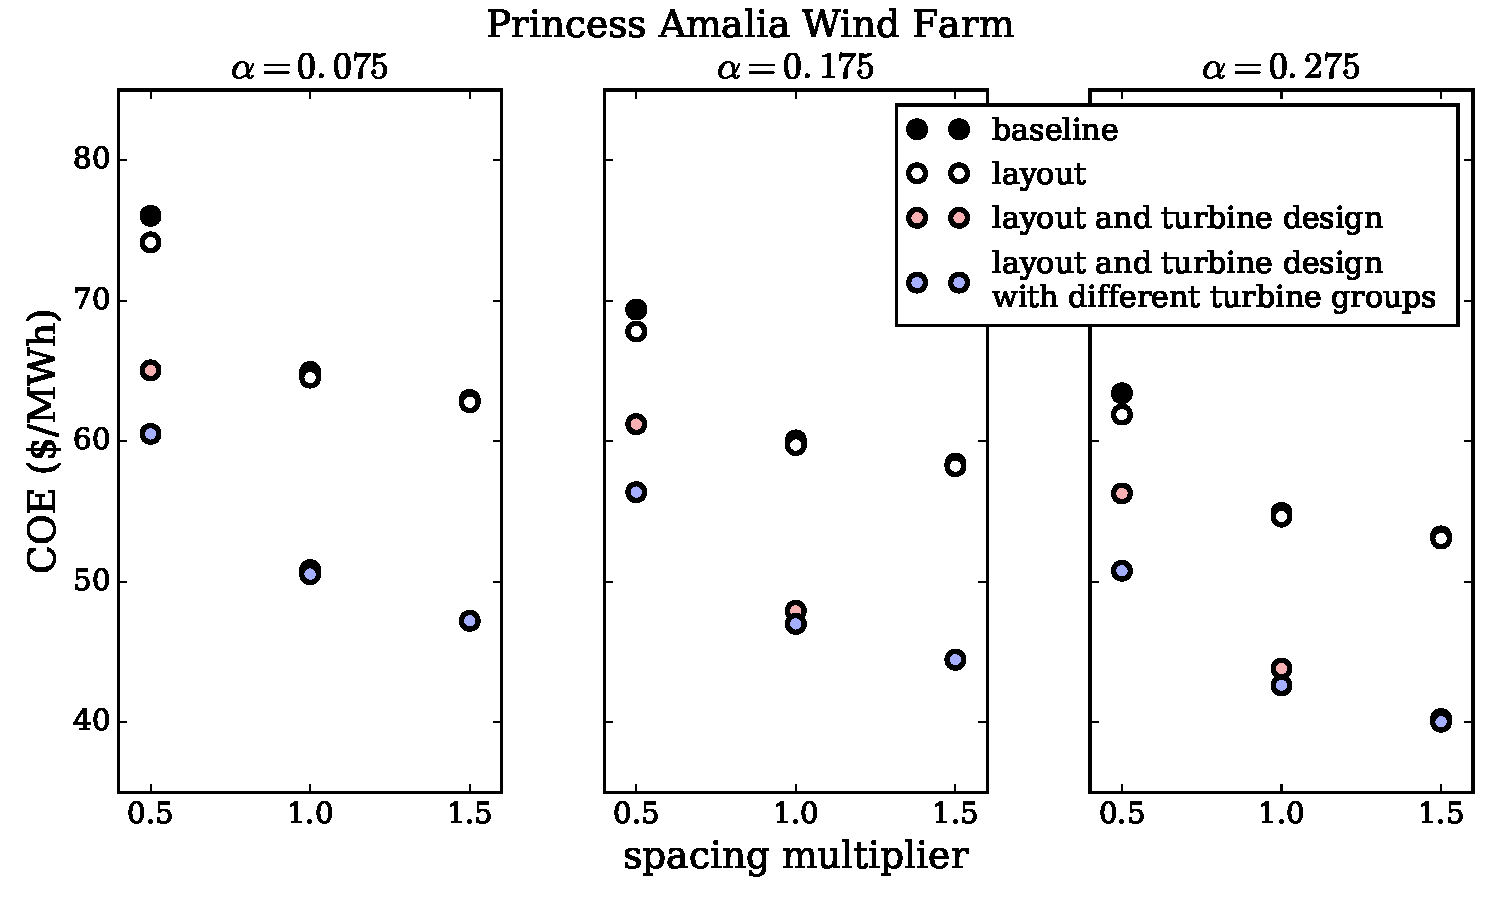
\includegraphics[width=\textwidth]{Figures/amalia_results.pdf}
%   \caption{\label{amalia_results} The optimal COE results for the Princess Amalia wind farm layout with 60 turbines. Each of the subfigures corresponds to optimization runs with a different shear exponent, from right to left $\alpha=0.075,0.175,0.275$. With in each subfigure, the x axis shows the size of the wind farm through the spacing multiplier, from right to left $\beta=0.5,1.0,1.5$. The different points represent the baseline, layout optimization, layout and turbine design optimization with homogeneous turbine design throughout the farm, and layout and turbine design optimization with two different turbine design groups.}
% \end{figure}

% \begin{center}
% \captionof{table}{}\label{tab:amalia}
% \begin{tabularx}{\textwidth}{|X|c|c|c|c|c|c|c|c|c|}
% \hline
% \multicolumn{10}{|c|}{\textbf{Princess Amalia: Percent COE Decrease from Baseline}}\\
% \hline
%  & \multicolumn{3}{c|}{$\alpha=0.075$} & \multicolumn{3}{c}{$\alpha=0.175$} & \multicolumn{3}{|c|}{$\alpha=0.275$}\\
% \hline
% optimization case & $\beta\myeq0.5$ & $\beta\myeq1.0$ & $\beta\myeq1.5$ & $\beta\myeq0.5$ & $\beta\myeq1.0$ & $\beta\myeq1.5$& $\beta\myeq0.5$ & $\beta\myeq1.0$ & $\beta\myeq1.5$\\
% \specialrule{.2em}{.1em}{.1em}
% layout & 2.48 & 0.62 & 0.26 & 2.25  & 0.55  & 0.30  & 2.39  & 0.48  & 0.27\\
% \hline
% coupled turbine design & 14.46  & 21.72  & 24.97  & 11.76  &  20.21 &  23.90 & 11.24  &  20.19 & 24.42\\
% \hline
% coupled turbine design: 2 groups & 20.41  & 22.17  & 24.98  & 18.74  & 21.75  & 23.88  & 19.92  &  22.34 & 24.79\\
% \hline
% \end{tabularx}
% \end{center}

% % The optimal rated power is low for the short, small turbines that won't produce as much energy, and larger for the taller, larger rotors that are capable of producing much more energy.

% \begin{figure}[htbp]
%   \centering
%   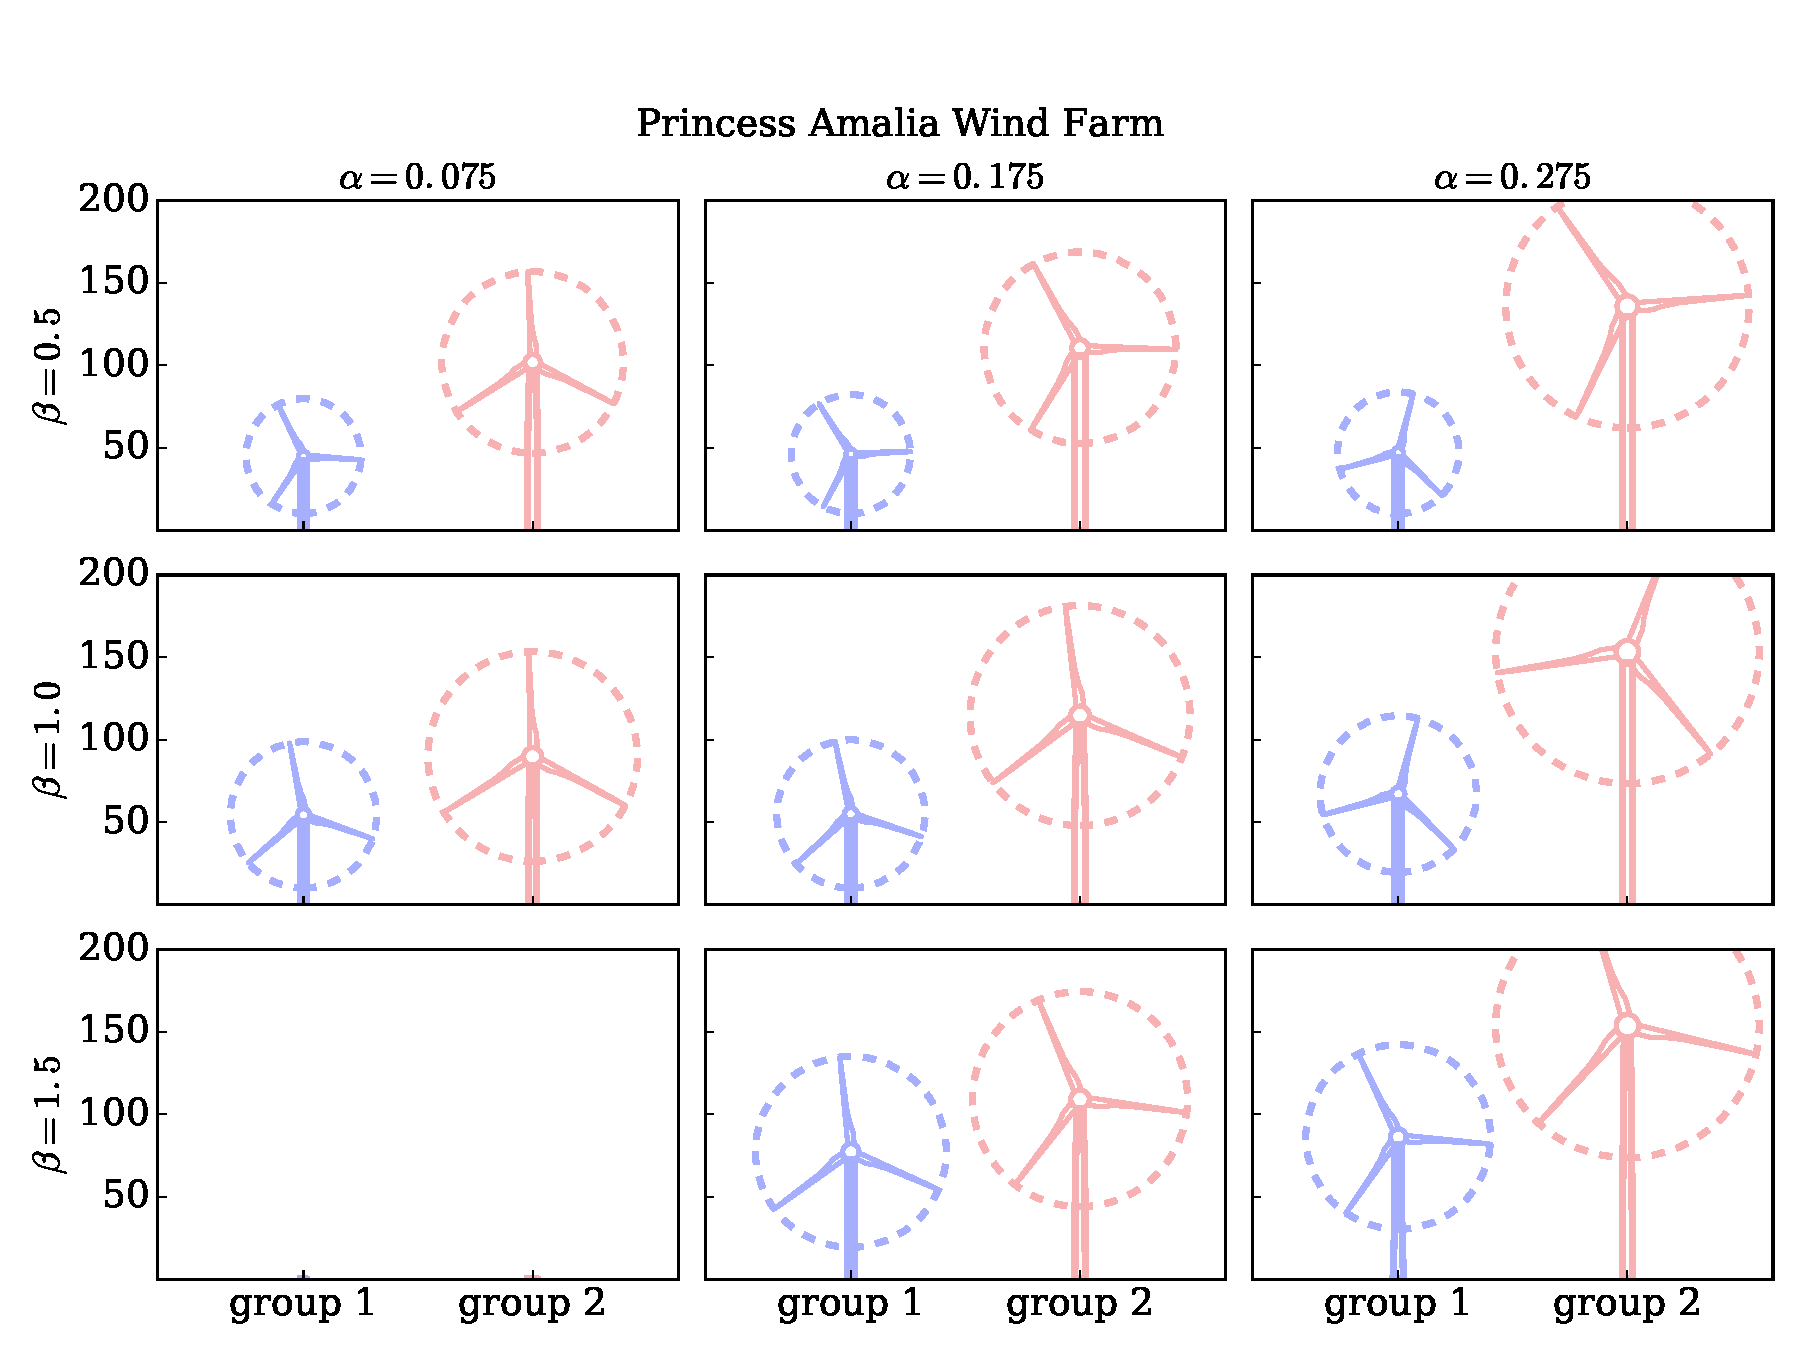
\includegraphics[trim={0.5cm 0.3cm 0.3cm 1.75cm},clip,width=\textwidth]{Figures/turbineSizesAmalia.pdf}
%   \caption{\label{amalia_turbines} The optimal turbine heights and rotor diameters for the optimization runs with coupled layout and turbine design with two different turbine design groups for the Princess Amalia wind farm. Each column shows a different shear exponent, with $\alpha=0.075,0.175,0.275$ from left to right. Each row shows a different farm spacing multiplier, with $\beta=0.5,1.0,1.5$ from top to bottom.}
% \end{figure}

% \begin{figure}[htbp]
%   \centering
%   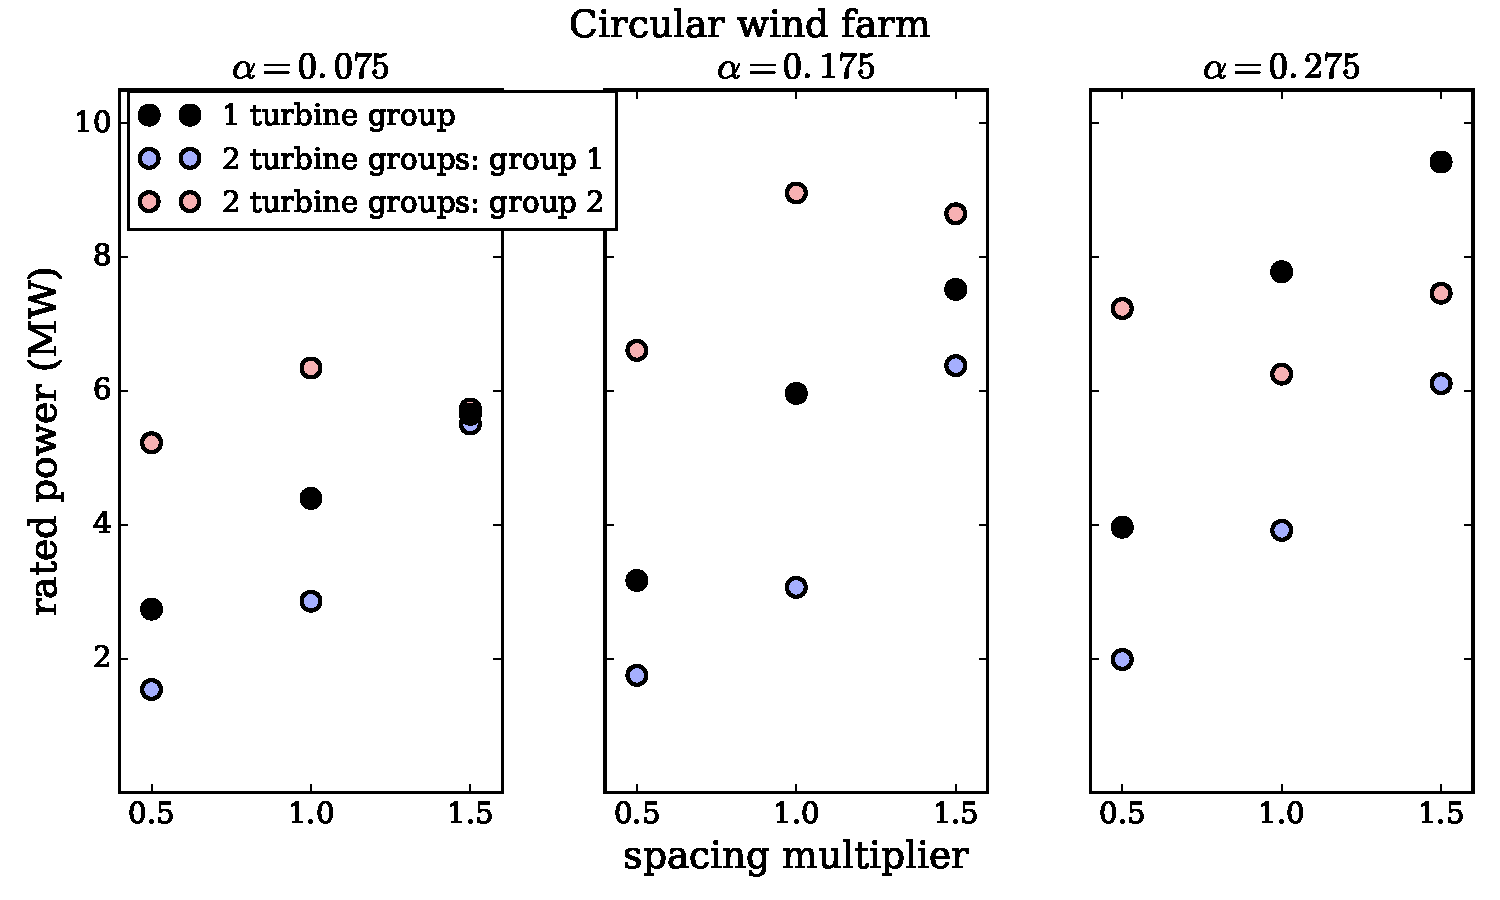
\includegraphics[trim={0.9cm 0cm 1.5cm 0cm},clip,width=\textwidth]{Figures/amaliaPowers.pdf}
%   \caption{\label{amalia_power} The optimal rated powers of each group for the optimization runs with coupled layout and turbine design with two different turbine design groups for the Princess Amalia wind farm. The three subfigures show a different shear exponent, with $\alpha=0.075,0.175,0.275$ from left to right. within each subfigure, the x axis shows different farm spacing multipliers, with $\beta=0.5,1.0,1.5$ from left to right.}
% \end{figure}




